\documentclass{article}
\usepackage[utf8]{inputenc}
\usepackage{hyperref}
\usepackage{amsmath}
\usepackage{amsfonts}
\usepackage{graphicx}
\usepackage{enumitem}
\usepackage{wrapfig}
\graphicspath{ {./images} }


\title{Freshman Physics}
\author{
    Tan Chien Hao\\
    \texttt{www.tchlabs.net}\\
    \texttt{Telegram @tch1001}
    % new collaborators add your name and contact here!
}

\date{\today}
\begin{document}
\newif\ifpaper

% TOGGLE ANSWER HERE
\paperfalse 

\maketitle

Updated notes are available at \url{https://bit.ly/3E6SuwA}. Please inform me of any errors. Feel free to message me to explain something in greater detail :) I also run a weekly SJPO / SPhO class if you're interested.
\tableofcontents

\section{Math: Functions}
Lecture: \url{https://youtu.be/-Ia9Wv5USaE}\\[10pt]
Functions are maps from one set to another set. We denote them as $f: A \rightarrow B$ or $f(x) \in B$ where $x\in A$. \\
\\
Examples of functions $f: \mathbb R \to \mathbb R$:
\begin{itemize}
    \item Particle's x coordinate $x(t) = 5 \sin (2t)$
    \item Particle's x component of velocity $v_x(t) = 10 \cos (2t)$
    \item Particle's x component of acceleration $a_x(t) = - 20 \sin (2t)$
    \item Potential Energy of spring mass system $U(x) = \frac{1}{2} k(x-x_0)^2$
    \item Current flowing through Resistor Capacitor circuit $I(t) = I_0 e^{-{t}/{RC}}$
    \item Kinetic Energy in terms of speed $T(|\vec{v}|) = \frac{1}{2} m |\vec{v}|^2$
\end{itemize}
\leavevmode \\
Examples of functions $f: \mathbb R \to \mathbb R^3$:
\begin{itemize}
    \item Particle path in 3D $\vec{s}(t) = \left(\begin{array}{l}
         x(t) \\
         y(t) \\
         z(t) 
    \end{array}\right) $
\end{itemize}
\leavevmode \\
Examples of functions $f: \mathbb R^3 \to \mathbb R$:

\begin{itemize}
    \item Gravitational Potential $\phi(x,y,z) = -\frac{GM}{\sqrt{x^2+y^2+z^2}}$
    \item Electric Potential Energy $\phi(\vec{r}) = -\frac{kQq}{|\vec{r}|}$. The arrow above $\vec{r}$ means it is a vector (more on this later)
    \item Temperature $T(\vec{r})$
\end{itemize}
\leavevmode \\
Examples of functions $f: \mathbb R^3 \to \mathbb R^3$:

\begin{itemize}
    \item Gravitational Force $\vec{F}(x,y,z) = -\frac{GMm}{(x^2 + y^2 + z^2)^{3/2}} \left(\begin{array}{l}
x \\
y \\ 
z
\end{array}\right)$
    \item Electrostatic Force $\vec{F}(\vec{r}) = \frac{kQq}{|\vec{r}|^2} \hat{r}$. The hat above $\hat{r}$ means it is a unit vector (scaled $\vec{r}$ to have length $1$).
\end{itemize}

\section{Math: Differentiation}
You probably know how to calculate the gradient of a linear (aka straight) graph.
$$m = \frac{y_1 - y_0}{x_1 - x_0}$$
This works if the graph is linear, i.e. $y=mx+c$. But what happens if the graph is not linear? e.g. $y = x^2$. How can we calculate the gradient of this curvy graph? Answer is \textbf{Differentiation}.

(Most) functions can be differentiated \textbf{with respect to} their parameters. \textbf{Algebraically}, differentiation involves following a set of rules. \textbf{Geometrically}, differentiation is the slope of the tangent line to the function's graph. 

\subsection{Geometric Intuition}
Lecture: \url{https://youtu.be/JYnXMoB288Q} \\[10pt]
\url{https://www.desmos.com/calculator/b6ts3ls1zf} Desmos visualization. Given a function $f(x)$, here's what the derivative $\frac{d}{dx}f = \frac{df}{dx} = f'(x)$ means:
\begin{itemize}
    \item Draw the graph $y=f(x)$.
    \item For each $x = x_0$ value, find the point on the graph $(x_0,f(x_0))$.
    \item Draw a (straight) tangent line to the graph at that point.
    \item Calculate the gradient of that tangent line.
    \item This gradient is the "derivative of $f$ \textbf{at }$x=x_0$".
    \item If you chose a different $x=x_1$ value, you would get a different value for gradient, and that would be "derivative of $f$ \textbf{at }$\mathbf{x=x_1}$".
    \item So the derivative of a function $f(x)$ is another function $f'(x)$.
\end{itemize}
\subsection{Algebraic Calculations}
Lecture: \url{https://youtu.be/QpSQmggia74} \\[10pt]
From the above geometric explanation, one can calculate the derivative of $f(x) = x^2$ to be $f'(x) = 2x$. This method of differentiation is called "from first principles".
\begin{align*}
f^{\prime}(x) & =\lim _{h \rightarrow 0} \frac{f(x+h)-f(x)}{h} \\
& =\lim _{h \rightarrow 0} \frac{\left((x+h)^2\right)-\left(x^2\right)}{h} \\
& =\lim _{h \rightarrow 0} \frac{x^2+2 h x+h^2-x^2}{h} \\
& =\lim _{h \rightarrow 0} \frac{2 h x+h^2}{h} \\
& =\lim _{h \rightarrow 0} \frac{h(2 x+h)}{h} \\
& =\lim _{h \rightarrow 0} 2 x+h \\
& =2 x
\end{align*}

Lecture: \url{https://youtu.be/Zg_6w0urW5Q} \\[10pt]
One can use first principles to derive the following rules of differentiation for common functions:

\begin{itemize}
    \item Linearity (Adding) 
    \begin{align}
        \frac{d}{dx} [f(x) + g(x)] &= \frac{df}{dx} + \frac{dg}{dx} \\
    \frac{d}{dx} [c f(x)] &= c \frac{df}{dx}
    \end{align}
    \item Polynomial $$ \frac{d}{dx} x^n = nx^{n-1} $$
    \item Trigonometry \begin{align}
        \frac{d}{dx} \sin(x) & = \cos(x) \\
        \frac{d}{dx} \cos(x) & = -\sin(x)
    \end{align}
    \item Exponential $$\frac{d}{dx} e^x = e^x$$
    \item Product Rule $$\frac{d}{dx} [f(x) g(x)] = f(x) \frac{dg}{dx} + g(x) \frac{df}{dx}$$
    \item Chain Rule $$\frac{d}{dx} f(y(x)) = \frac{df}{dy} \frac{dy}{dx}$$
\end{itemize}


\subsubsection{Finding Maximum / Minimum}
Lecture: \url{https://youtu.be/McI7tyS_BCo} \\[10pt]
When the function $f(x)$ has a maximum $x_{\text{max}}$, the derivative at that maximum point is zero $$\left. \frac{df}{dx} \right|_{x_{\text{max}}} = 0$$
Likewise for minimum.\\[10pt]
So if the function has $0$ derivative at some $x=x_0$, how do we determine if it's a maximum or minimum point? We can perform the 2nd derivative test.\\

\begin{align}
    \left. \frac{d^2 f}{dx^2} \right|_{x_0} > 0 &: \text{Minimum}\\
    \left. \frac{d^2 f}{dx^2} \right|_{x_0} < 0 &: \text{Maximum}\\
    \left. \frac{d^2 f}{dx^2} \right|_{x_0} = 0 &: \text{Not enough information to conclude}
\end{align}

\subsection{Exercises}
Try differentiating the following functions with respect to $x$ or $t$. You can check your answer against Wolfram Derivative Calculator \url{https://www.wolframalpha.com/calculators/derivative-calculator/}.

\begin{itemize}
    \item $\frac{d}{dx} x^4 + x^2$
    \item $\frac{d}{dt} 5t + 3$
    \item $\frac{d}{dx} \frac{1}{x}$
    \item $\frac{d}{dt} \sin (2t)$
    \item $\frac{d}{dt} e^{-5t}$
    \item $\frac{d}{dx} \tan x$
\end{itemize}
\textbf{Extra:} If the function of \textbf{multiple variables} is differentiated, it's called \textbf{multivariate calculus}. Multivariate calculus is used in Electromagnetism (Maxwell's Equations).



\section{Math: Integration / Anti-Differentiation }

Geometrically, (definite) integration gives you the area under the graph. Algebraically, there are a few techniques for common functions but integration is tricky in general. 

\subsection{Indefinite Integration / Antiderivative}
Lecture: \url{https://youtu.be/Nm8WVmlnxN8} \\[10pt]
Q: If I give you a function $f(x)$ and told you that it's derivative is $f'(x) = 2x + 1$, can you find out what $f(x)$ is? \\
A: $f(x) = x^2 + x + C$ where $C$ is an arbitrary constant. Why are there multiple answers?\\[10pt]
Mathematically, we say $$\int 2x + 1\ dx = x^2 + x + C$$
More generally, $$\int f'(x) dx = f(x) + C$$

\subsection{Exercises}
You can check whether you are correct by putting your answer in the derivative calculator and checking if you get the function to be integrated!
\begin{itemize}
    \item $\int 5\ dx$ 
    \item $\int \left( \int -10 dt \right) dt$
    \item $\int \sin(5t) \ dt$
    \item $\int (1/x^2) dx$
\end{itemize}


\textbf{Extra:} Some functions have antiderivatives that cannot be even expressed analytically, such as $$\int e^{-x^2} dx$$

\subsection{Definite Integration / Area under graph}
Lecture: \url{https://youtu.be/0IHvAyIaY44}\\[10pt]
Lecture (Side Note about Signed Area): \url{https://youtu.be/g_tr0sqJxM8}\\[10pt]
You can calculate the area under a curve by performing a \textbf{definite} integral.
\begin{align}
    \text{Area under }f'(x)\text{ from }(x=a)\text{ to }(x=b) &= \int_a^b f'(x)\ dx  \\
    &= \left[f(x) + C\right]^b_a \\
    &= f(b) - f(a)
\end{align}

Q: Why does the arbitrary constant $C$ not appear in the formula for area under the graph? 

A: It cancels out: $[f(b) + C] - [f(a) + C]$. Can you imagine this graphically? 

\subsection{Exercises}
Lecture: \url{https://youtu.be/ZlvM1BZRFXo}\\[10pt]
\begin{itemize}
    \item Energy in Spring
        $$\int_0^x kr\ dr$$
    \item Energy in Capacitor
        $$\int_0^Q \frac{q}{C} dq$$
    \item Gravitational Potential
        $$\int_{r}^{\infty} \frac{1}{x^2} dx$$
\end{itemize}

\section{Physics: Kinematics}
Lecture: \url{https://youtu.be/c527UZUQM0s} \\[10pt]
After picking a direction which you define as "increasing x direction" as well as an origin for x, you can start describing 1D motion $x(t)$.\\
\\
If you want to describe 2D motion, pick a perpendicular y-axis. \\
\\
If you want to describe 3D motion, z-axis is defined using RHR (for the cross product).
\subsection{Path of Particle / Object}
Lecture: \url{https://youtu.be/vszG98TSd6Q}\\[10pt]
Mathematically, paths are functions $\vec{s}(t)$ of a parameter $t$ representing time. 
\begin{itemize}
    \item In 1D motion, $x(t)$ 
    \item In 2D motion, $x(t),\ y(t)$
    \item In 3D motion, $x(t),\ y(t),\ z(t)$
\end{itemize}
To understand an object's behaviour, our goal is to solve for the 3 functions $x(t),\ y(t),\ z(t)$, meaning we obtain a formula like $y(t) = 2 t - 5 t^2$. Knowing where the object is at every snapshot in time allows us to calculate it's velocity $\vec{v}(t)$, it's acceleration $\vec{a}(t)$, how long it'll take to travel from A to B ($\Delta t = t_B - t_A$), the forces $\vec{F}(\vec{s}(t))$ acting on it at any time, etc.

\subsection{SUVAT}
\begin{align}
v(t)&=u+a t \label{eq:vuat} \\
s(t)&=u t+\frac{1}{2} a t^2 \label{eq:suat}\\
 v(s)^2&=u^2+2 a s \label{eq:vuas} \\
 s(t)&=\frac{v(t)+u}{2} t \label{eq:svut}\\
 s(t)&=v(t) t-\frac{1}{2} a t^2 \label{eq:svat}
\end{align}
SUVAT laws can be derived from calculus with the following definitions.\\[10pt]
Let $s(t)$ be the function representing the particle's (1D) coordinate.
\begin{align}
    v(t) &:= \frac{ds}{dt} \\
    a(t) &:= \frac{dv}{dt} = \frac{d^2 s}{dt^2}
\end{align}
\\
If acceleration is constant, i.e. $$a(t) = \frac{d^2 s}{dt^2} = a_0$$ for some constant $a_0$, then one can integrate the above equation once and twice to get 2 of the SUVAT laws 

\begin{align}
    v(t) &= a_0 t + v_0 \\
    s(t) &= \frac{1}{2} a_0 t^2 + v_0 t + s_0 
\end{align}
\\
where we identify $a_0 \equiv a$, $v_0 \equiv u$, $s_0 \equiv 0$ to match \ref{eq:vuat} and \ref{eq:suat}.\\
\\
The other 3 equations can be obtained from the first 2 with a bit of algebra.\\

\subsection{Geometric Intuition}
SUVAT can be visualized as an area of a trapezium in the $v\text{-}t$ graph. [Demonstrate in class]


\subsection{Exercises}
\begin{samepage}
\subsubsection{SJPO 2015 General Round Q13}
Lecture: \url{https://youtu.be/j9qWyWCTjrM} \\[10pt]
An object is travelling on a straight path and exhibiting a constant acceleration $a$ starts off with an initial velocity $v=2.0 \mathrm{~ms}^{-1}$. It has traversed $4.5 \mathrm{~m}$ in the third second (from $t=2$ to $t=3$), its acceleration $a$ is
\begin{itemize}\item[](A) $0.5 \mathrm{~ms}^{-2}$
\item[](B) $1.0 \mathrm{~ms}^{-2}$
\item[](C) $1.5 \mathrm{~ms}^{-2}$
\item[](D) $2.0 \mathrm{~ms}^{-2}$
\item[](E) $2.5 \mathrm{~ms}^{-2}$
\end{itemize}
Ans: \ifpaper B \fi
\end{samepage}
\\[20pt]
% SJPO 2015 General Round Q28: The Moon is approximately $380,000 \mathrm{~km}$ from Earth. The time a laser light beam takes to travel from the Earth to the Moon and back is most nearly
% \begin{itemize}\item[](A) 2 microseconds.
% \item[](B) 2 milliseconds.
% \item[](C) 2 seconds.
% \item[](D) 2 minutes.
% \item[](E) 2 hours. 
% Ans:C
\begin{samepage}
\subsubsection{SJPO 2016 General Round Q8}
Lecture: \url{https://youtu.be/Q3ZbXLegdos} \\[10pt]
A train moving on straight horizontal tracks slows down from $66 \mathrm{~ms}^{-1}$ to $22 \mathrm{~ms}^{-1}$ at a constant rate of $2.0 \mathrm{~ms}^{-2}$. What distance does it travel while slowing down?
\begin{itemize}
\item[](A) $490 \mathrm{~m}$
\item[](B) $650 \mathrm{~m}$
\item[](C) $740 \mathrm{~m}$
\item[](D) $970 \mathrm{~m}$ 
\item[](E) $1100 \mathrm{~m}$ \end{itemize}
Ans: \ifpaper D \fi
\end{samepage}
\\[20pt]
% SJPO 2016 General Round Q9 A (Projectile Motion)
% SJPO 2016 General Round Q11 E (Projectile)
\begin{samepage}
\subsubsection{SJPO 2018 General Round Q10} 
Lecture: \url{https://youtu.be/gLHMK0g8JYc} \\[10pt]
The position of an object moving along a linear track is plotted as a function of time. It started from rest and underwent a positive acceleration for some time, followed by a constant velocity. Which of the following graphs correctly shows this situation?\\
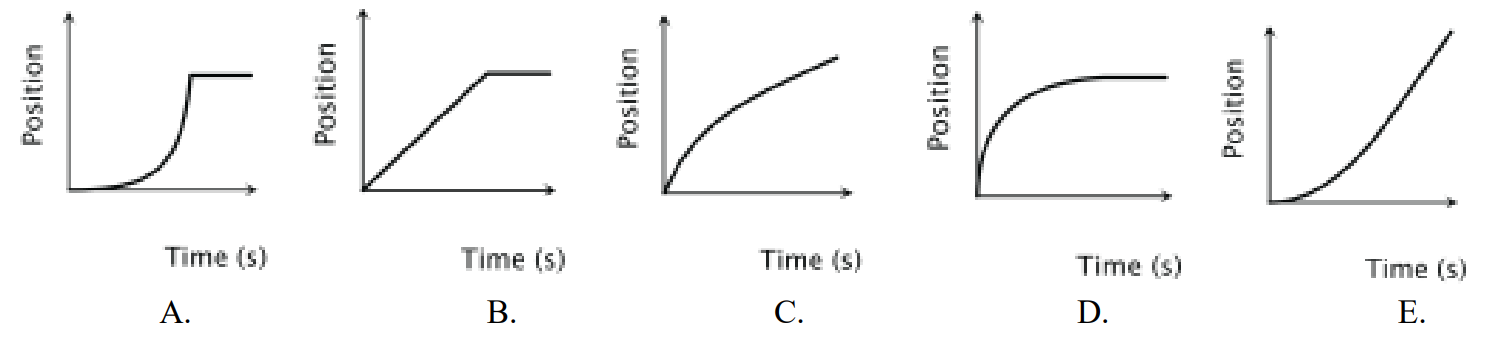
\includegraphics[width=\linewidth]{2018q10.png}\\
Ans: \ifpaper E \fi\\
\end{samepage}


\subsubsection{SJPO 2018 General Round Q16 \& Q17}
Lecture: \url{https://youtu.be/5M1mQjZJWI4} \\[10pt]
A car travels along a straight road with the speed shown by the 
v-t graph. \\ 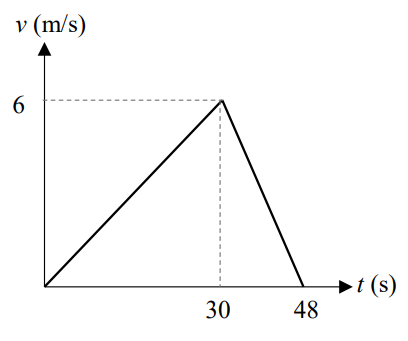
\includegraphics[width=0.5\linewidth]{images/2018q16.png} \\
\\
\begin{samepage}
16. What is the acceleration of the car from $t=30$ to $t=48 \mathrm{~s}$ ?
\begin{itemize}
\item[] (A) $-54 \mathrm{~m} / \mathrm{s}^2$ 
\item[] (B) $\quad 48 \mathrm{~m} / \mathrm{s}^2$ 
\item[] (C) $-3.0 \mathrm{~m} / \mathrm{s}^2$ 
\item[] (D) $\quad 3.0 \mathrm{~m} / \mathrm{s}^2$
\item[] (E) $-0.33 \mathrm{~m} / \mathrm{s}^2$\end{itemize}
Ans: \ifpaper E \fi
\end{samepage}
\\[20pt]
\begin{samepage}
17. What is the total displacement of the car after $48 \mathrm{~s}$ ?
\begin{itemize}
\item[] (A) $36 \mathrm{~m}$
\item[] (B) $48 \mathrm{~m}$
\item[] (C) $144 \mathrm{~m}$
\item[] (D) $180 \mathrm{~m}$
\item[] (E) $210 \mathrm{~m}$ 
\end{itemize}
Ans: \ifpaper C \fi\\
\end{samepage}
\\
\begin{samepage}
\subsubsection{SJPO 2017 General Round Q1} 
Lecture: \url{https://youtu.be/TW3sIS0lprI} \\[10pt]
An electron in a vacuum, starting from rest falls $5 \mathrm{~cm}$ near the surface of the earth. Considering only the gravitational force acting on the electron, how long does it take for the electron to travel $5 \mathrm{~cm}$?
\begin{itemize}
\item[] (A) $\quad 0.1 \mathrm{~s}$
\item[] (B) $\quad 0.03 \mathrm{~s}$
\item[] (C) $\quad 0.01 \mathrm{~s}$
\item[] (D) $\quad 0.001 \mathrm{~s}$
\item[] (E) $\quad 0.0001 \mathrm{~s}$
\end{itemize}
Ans: \ifpaper A \fi
\end{samepage}
% SJPO 2018 General Round Q18 C

\subsection{1D Dynamics}
Lecture: \url{https://youtu.be/xWJjy_5M4lA} \\[10pt]
If we know the acceleration as a function of time $a(t)$, as well as the initial velocity $v(t=0) \equiv v_0$ and position $s(t=0) \equiv s_0$, then we can integrate $a(t)$ twice to get the position as a function of time 
$$s(t) = \int \left(\int a(t)\ dt\right)\ dt$$

To obtain this $a(t)$, we use Newton's 2nd law 
$$F_{\text{net}}(t) = \frac{d(mv)}{dt} = m \frac{dv}{dt} + v \frac{dm}{dt}$$
In (most) cases where $m(t)$ is a constant wrt time, 
$$F_{\text{net}}(t) = ma(t)$$



\subsection{Extra: $v^2 = u^2 + 2as$ Connection with Work Energy Theorem}
Lecture: \url{https://youtu.be/1Z9V-1STA_Y} \\[10pt]
$v^2 = u^2 + 2as$ is slightly special because it is related to "work energy theorem" in dynamics. One can derive it by integrating $a(t)$ wrt $s(t)$ instead of $t$ 
\begin{align}
    \frac{d^2 s}{dt^2} &= a_0 \\
    \frac{d}{dt} \left(\frac{ds}{dt}\right) \frac{ds}{dt} dt &= a_0 ds \\
    \frac{1}{2} \frac{d}{dt} \left( v(t)^2 \right) dt &= a_0 ds \\
    \int_{t_A}^{t_B} \frac{1}{2} \frac{d}{dt} \left( v(t)^2 \right) dt &= \int_{s_A}^{s_B} a_0 ds \\
    \int_{v_A}^{v_B} \frac{1}{2} d\left( v^2 \right) &= a_0 (s_B - s_A) \\
    \frac{1}{2} (v_B^2 - v_A^2) &= a_0 (s_B - s_A) \\
    v_B^2 &= v_A^2 + 2a_0(s_B - s_A)
\end{align}

where we identify $v_B \equiv v$, $v_A \equiv u$, $s_B \equiv s$, $s_A \equiv 0$, $a_0 \equiv a$ to match \ref{eq:vuas}.
\\
 

\section{Math: 3D Vectors}

I made some H2 math videos on vectors 
\begin{itemize}
    \item \url{https://youtu.be/zohpKrmHkc0} Adding, scaling, subtraction of vectors
    \item \url{https://youtu.be/LhXac_HUw-0} Dot product
    \item \url{https://youtu.be/1qruXfQRQJU} Cross product
\end{itemize}
\leavevmode \\
In order to describe 3D motion we have 3 functions $x(t),y(t),z(t)$. To avoid writing three equations, we often package them into a position vector.
\begin{align}
    \vec{r}(t) = \left(
    \begin{array}{c}  
         x(t) \\
         y(t) \\
         z(t)
    \end{array}
    \right)
\end{align}

Geometrically, a vector can be thought of as an arrow. It is the "displacement between 2 points in 3D space", and points in a particular \textbf{direction} and has a \textbf{length/magnitude}. 

\subsection{Vector Operations}
\subsubsection{Adding}
Algebraically, just add each component individually
$$\left(
    \begin{array}{c}  
         x_1 \\
         y_1 \\
         z_1
    \end{array}
    \right) + \left(
    \begin{array}{c}  
         x_2 \\
         y_2 \\
         z_2
    \end{array}
    \right) = \left(
    \begin{array}{c}  
         x_1 + x_2 \\
         y_1 + y_2 \\
         z_1 + z_2
    \end{array}
    \right) 
$$
Geometrically, \\
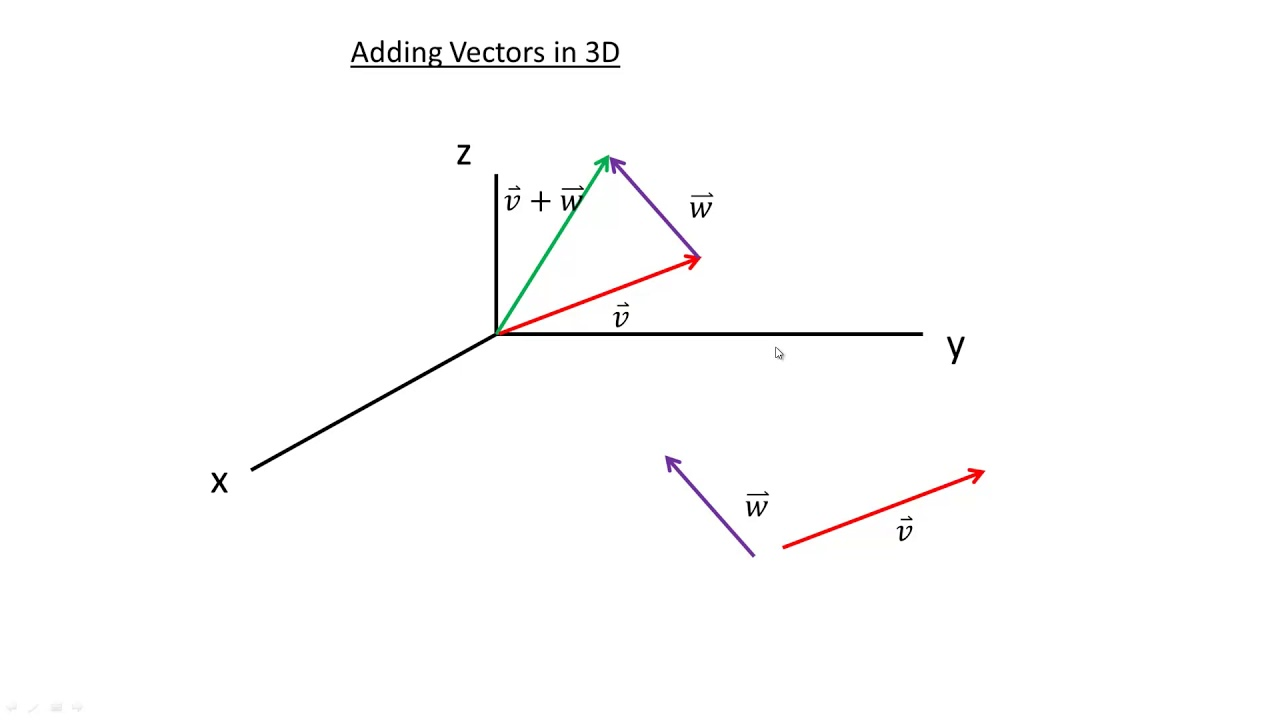
\includegraphics[width=\linewidth]{images/addingvectors.jpg}
\subsubsection{Scaling}
Algebraically, scale each component individually
$$
\lambda \left(
    \begin{array}{c}  
         x \\
         y \\
         z
    \end{array}
    \right) = \left(
    \begin{array}{c}  
         \lambda x \\
         \lambda y \\
         \lambda z
    \end{array}
    \right)
$$

Geometrically, if you scale a vector by a positive real number, direction stays the same but length is changed. \\
\begin{center}
    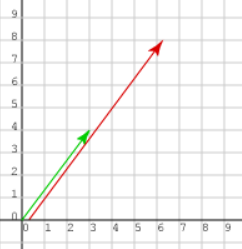
\includegraphics[width=0.3\linewidth]{images/scalingvector.png}
\end{center}
If scaled by a negative number, the direction flips (and length changes too).

\subsubsection{Length}
Algebraically, length is calculated using Pythagoras' theorem.
$$\left| \left(
    \begin{array}{c}  
         x \\
          y \\
          z
    \end{array}
    \right) \right| = \sqrt{x^2 + y^2 + z^2}
    $$

\subsubsection{Dot Product}
Dot product takes 2 vectors and outputs a single real number.
$$\left(
    \begin{array}{c}  
         x_1 \\
         y_1 \\
         z_1
    \end{array}
    \right) \cdot \left(
    \begin{array}{c}  
         x_2 \\
         y_2 \\
         z_2
    \end{array}
    \right) = x_1 x_2 + y_1 y_2 + z_1 z_2 
$$
Geometrically, dot product is a measure of how similar the direction of the 2 vectors are.
$$\vec{a} \cdot \vec{b} = |\vec{a}| |\vec{b}| \cos \theta $$
where $\theta$ is the angle between the 2 vectors.\\[10pt]
The dot product is used to define 
\begin{itemize}
    \item Work Done $W.(D) = \int \vec{F} \cdot d\vec{r}$
    \item Magnetic Flux $\Phi = \int \vec{B} \cdot d\vec{A}$
\end{itemize}

\subsubsection{Cross Product}
Cross product takes 2 vectors and outputs another vector.
$$\left(
    \begin{array}{c}  
         x_1 \\
         y_1 \\
         z_1
    \end{array}
    \right) \times \left(
    \begin{array}{c}  
         x_2 \\
         y_2 \\
         z_2
    \end{array} 
    \right) = \left(
    \begin{array}{c}  
         y_1 z_2 - z_1 y_2 \\
         z_1 x_2 - x_1 z_2 \\
         x_1 y_2 - y_1 x_2
    \end{array}
    \right)
$$

Geometrically, the length of the cross product is the area of the parallelogram. The direction of the cross product is perpendicular (following right hand rule). \\
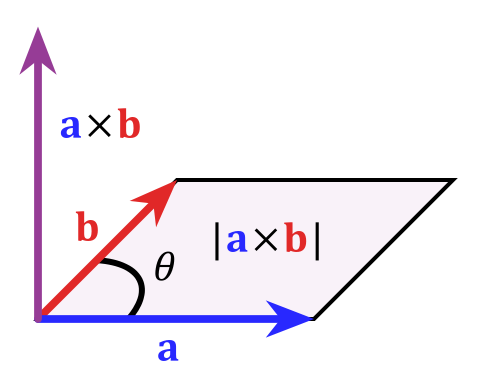
\includegraphics[width=0.49\linewidth]{images/crossproduct.png}
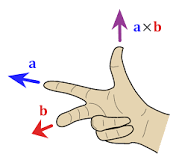
\includegraphics[width=0.49\linewidth]{images/crossproduct2.png}\\
The cross product is used to define 
\begin{itemize}
    \item Torque $\vec{\tau} = \vec{r} \times \vec{F}$
    \item Angular Momentum $\vec{L} = \vec{r} \times \vec{p}$
    \item Lorentz Force $\vec{F} = q(\vec{E} + \vec{v}\times \vec{B})$
    \item Poynting Vector $\vec{S}=\frac{1}{\mu_0} \vec{E} \times \vec{B}$
\end{itemize}
\subsubsection{Derivatives}
Also done component wise
$$\frac{d\vec{r}}{dt} = \frac{d}{dt}\left(
    \begin{array}{c}  
         x \\
         y \\
         z
    \end{array} 
    \right) = \left(
    \begin{array}{c}  
         dx/dt \\
         dy/dt \\
         dz/dt
    \end{array} 
    \right)
$$
\subsection{Basis Vectors}
We sometimes write a vector as 
\begin{align}
    \vec{r} &= \left(
    \begin{array}{c}  
         x(t) \\
         y(t) \\
         z(t)
    \end{array} 
    \right) \\
    &= x(t) \left(
    \begin{array}{c}  
         1 \\
         0 \\
         0
    \end{array} 
    \right) + y(t) \left(
    \begin{array}{c}  
         0 \\
         1 \\
         0
    \end{array} 
    \right) + z(t) \left(
    \begin{array}{c}  
         0 \\
         0 \\
         1
    \end{array} 
    \right)  \\
    &\equiv x(t) \hat{i} + y(t) \hat{j}  + z(t) \hat{k} 
\end{align}
Common synonyms for $\hat{i}$ are $\hat{x}$ and $\hat{e}_x$. The collection of vectors $\{ \hat i, \hat j, \hat k \}$ are called a set of \textbf{basis vectors}, which means that linear combinations of these vectors make up / span the set of all possible vectors. In particular, this set $\{ \hat i, \hat j, \hat k \}$ is called the \textbf{Cartesian coordinate basis}. In future, we will learn about other coordinate systems and other basis vectors.
\subsection{Exercises}
\begin{samepage}
\subsubsection{SJPO 2015 General Round Q11}
A force $\vec{F} = \vec{F}_1 + \vec{F}_2$ can be decomposed as the sum of 2 vectors $\vec{F}_1$ and $\vec{F}_2$. Only the magnitude of $\vec{F}_1$ and the direction of $\vec{F}_2$ are known. Which of the following is the most accurate statement?
\begin{itemize}
\item[](A) Only one combination of $\vec{F}_1$ and $\vec{F}_2$ exists.
\item[](B) There exists exactly two combinations of $\vec{F}_1$ and $\vec{F}_2$.
\item[](C) There exists infinite combinations of $\vec{F}_1$ and $\vec{F}_2$.
\item[](D) At least three combinations of $\vec{F}_1$ and $\vec{F}_2$ exist but the total number of combinations is finite.
\item[](E) Only one or two combinations of $\vec{F}_1$ and $\vec{F}_2$ exist.
\end{itemize}
Ans: \ifpaper E \fi
\end{samepage}
\begin{samepage}
\subsubsection{SJPO 2016 General Round Q21}
Initially, a $1\mathrm{~kg}$ box was sliding on frictionless surface at a constant velocity of $4\mathrm{~ms}^{-1}$ in the $\mathrm{x}$ direction. A constant force of $1\mathrm{~N}$ was applied on the box in a fixed direction for a time duration of $5\mathrm{~s}$. After $5\mathrm{~s}$ the speed of the box is $3\mathrm{~ms}^{-1}$. What is the magnitude of the change in momentum of the box?
\begin{itemize}
\item[](A) $1 \mathrm{kgms}^{-1}$
\item[](B) $2 \mathrm{kgms}^{-1}$
\item[](C) $3 \mathrm{kgms}^{-1}$
\item[](D) $4 \mathrm{kgms}^{-1}$
\item[](E) $5 \mathrm{kgms}^{-1}$
\end{itemize}
Ans: \ifpaper E \fi \\[10pt]
Extra: What are the possible directions of the applied force? 
\end{samepage}
\newpage
\section{Physics: Newtonian Mechanics}
The following quantities are scalars (real numbers)
\begin{itemize}
    \item mass $m$
    \item speed $|\vec{v}|$
    \item kinetic energy $E = \frac{1}{2} m|\vec{v}|^2$
    \item potential energy $U$
\end{itemize}
The following quantities are vectors
\begin{itemize}
    \item position $\vec{r}(t)$
    \item velocity $\vec{v}(t) \equiv \frac{d\vec{r}}{dt}$
    \item acceleration $\vec{a}(t) \equiv \frac{d^2\vec{r}}{dt^2}$
    \item force $\vec{F}(t)$
    \item momentum $\vec{p}(t) \equiv m\vec{v}(t)$
\end{itemize}
\leavevmode \\
\subsection{Newton's Three Laws}
\url{https://youtu.be/M6uYi0lcOvU}
Newton's 1st law defines what an inertial reference frame is: \textbf{In an inertial reference frame}, an object at rest remains at rest, or if in motion, remains in motion at a constant velocity unless acted on by a net external force.\\[10pt]
\textbf{In an inertial reference frame}, Newton's 2nd law
$$\vec{F}_{\text{net}} = \frac{d(m\vec{v})}{dt}$$
Newton's 3rd law 
$$\vec{F}_{\text{A on B}}(t) = -\vec{F}_{\text{B on A}}(t)$$

\subsection{Momentum \& Impulse}
\url{https://youtu.be/TiOSscc8TKw}
Change in a particle's momentum is equal to the impulse it experiences. \\[10pt]
Newton's 2nd law: Let $\vec{F}(t)$ be the net force on a particle, then
$$\vec{F}(t) = \frac{d\vec{p}}{dt}$$
Let's focus on one component of the vector equation (say $F_x, p_x$)
$$F_x(t) = \frac{dp_x}{dt}$$
Integrating both sides wrt time $t$ from $t=t_A$ to $t=t_B$ yields

\begin{align}
    \int_{t_A}^{t_B} F_x(t) dt &= \int_{t_A}^{t_B} \frac{dp_x}{dt} dt \\
    \int_{t_A}^{t_B} F_x(t) dt &= \int_{p_x(t_A)}^{p_x(t_B)} dp_x \\
    &= p_x(t_B) - p_x(t_A) \\
    &= \Delta p_x
\end{align}
If a particle experiences a force $\vec{F}(t)$ over a time period $t_A$ to $t_B$, it's ($x$-component of) momentum will change by $\Delta p_x = \int_{t_A}^{t_B} F_x(t) dt$.\\[10pt]
This is true for each component $x,y,z$ so actually it is a vector equation 
$$\Delta \vec{p} = \int_{t_A}^{t_B} \vec{F}(t) dt$$
The quantity on the right hand side is called \textbf{impulse}.

\subsection{Kinetic Energy \& Work}
\url{https://youtu.be/DYRDr_ADIAM}
Often in physics, it is unnecessary to know the exact path $x(t)$ of a particle. Sometimes, the question only requires us to know $v(t)$. \\[10pt]
Example: A particle of mass $m$ experiences a force $F(x(t)) = \frac{A}{x(t)^2}$. It starts at $x(0)=x_0,\ x_0 > 0$ with an initial speed of $v_0$ toward $x=0$. Where will the particle come to a rest? \\[10pt]
One way of solving this is to find the function $x(t)$ that satisfies $F=ma$
$$\frac{A}{x^2} = m \frac{d^2x}{dt^2}$$
This is a differential equation, which we will cover later. We realise we cannot integrate wrt $t$ because the LHS itself is a function of $t$ we do not know the expression for. We will actually integrate wrt $x(t)$. We need to massage the equation into a different form first.\\[10pt]
By chain rule,
\begin{align}
\frac{d}{d t}\left[\left(\frac{d x}{d t}\right)^2\right]&=2  \frac{d x}{d t} \frac{d^2 x}{d t^2} 
\end{align}
Substituting this back in and simplifying
\begin{align}
\frac{A}{x^2}&=\frac{m}{2 \frac{d x}{d t}} \frac{d}{d t}\left[\left(\frac{d x}{d t}\right)^2\right] \\
& =\frac{m}{2} \frac{d}{d x}\left[\left(\frac{d x}{d t}\right)^2\right] \\
& =\frac{m}{2} \frac{d}{d x} v^2 
\end{align}
Then integrating from the starting to the stopping point wrt $x$ instead of $t$,
\begin{align} 
\int_{x_0}^{x_{\text {stop }}} \frac{A}{x^2} d x&=\frac{m}{2} \int_{v_0^2}^{v_{\text {stop }}^2=0} d\left[\left(\frac{d x}{d t}\right)^2\right] \\
\left[-\frac{A}{x}\right]_{x_0}^{x_\text{stop}} &= \left[\frac{1}{2} m v^2\right]_{v^2=v_0^2}^{v^2=0} \\
\frac{A}{x_0}-\frac{A}{x_\text {stop }}&=-\frac{1}{2} m v_0^2 \\
\frac{A}{x_0}+\frac{1}{2} m v_0^2&=\frac{A}{x_\text {stop }} \label{eq:pepke}\\
x_{\text{stop}} &= A \left(\frac{A}{x_0}+\frac{1}{2} m v_0^2\right)^{-1}
\end{align}
The left hand side of Equation \ref{eq:pepke} is actually potential energy + kinetic energy. We will talk about potential energy in future, but for now we observe that integrating $F$ with respect to $x$ instead of $t$ was a useful trick. Generalizing this to a general force $F$,

\begin{align}
    F &= ma \\
    \int_{x_A}^{x_B} F dx &= m \int_{x_A}^{x_B} a dx 
\end{align}
Claim: $a\ dx = v\ dv$. Proof: 
\begin{align}
v\ dv
& = \frac{1}{2} d\left(v^2\right) \\
& =\frac{1}{2} \frac{d}{d t}\left(v^2\right) d t \\
& =\frac{1}{2} 2 v a\ d t \\
& =a\ v\ d t \\
& =a \ d x
\end{align}
So by a change in variables, $a\ dx = v\ dv$. 
\begin{align}
    \int_{x_A}^{x_B} F dx &= m \int_{x_A}^{x_B} a dx \\
    &= m \int_{v_A}^{v_B} v dv \\
    &= \frac{1}{2} m \left[v^2\right]_{v_A}^{v_B} \\
    &= \frac{1}{2} m v_B^2 - \frac{1}{2} mv_A^2 \\
    &= \Delta K.E.
\end{align}
In other words, if a particle experiences a force $F(x)$ over a distance interval from $x_A$ to $x_B$, it's change of kinetic energy $\Delta\left(\frac{1}{2}mv^2\right)$ is given by $$\Delta K.E. = \int_{x_A}^{x_B} F(x)\ dx$$
which we call the \textbf{work done} on the particle. This is the \textbf{Work Energy theorem}.\\[10pt]
Extra: Mathematically, what we have actually done is we have transformed a 2nd order ODE $a(x)$ into a 1st order ODE $v(x)$, which should be easier to integrate in general.

\section{Physics: Projectile Motion}
\url{https://youtu.be/-Yq6wzXTU84}
\begin{align}
\vec{F}_{\text{net}} &= m \vec{a} \\
\Rightarrow \left(
    \begin{array}{c}  
         0 \\
         -mg \\
         0
    \end{array} 
    \right) &= m \left(
    \begin{array}{c}  
         d^2x/dt^2 \\
         d^2y/dt^2 \\
         d^2z/dt^2
    \end{array} 
    \right)
\end{align}
Integrating twice with respect to time $t$,
\begin{align}
    \left(
    \begin{array}{c}  
         x(t) \\
         y(t) \\
         z(t)
    \end{array} 
    \right) = \left(
    \begin{array}{c}  
          {u}_x t + {r_0}_x\\
         -\frac{1}{2}gt^2 + {u}_y t + {r_0}_y\\
          {u}_z t + {r_0}_z
    \end{array} 
    \right)
\end{align}
We need to know the initial position $\vec{r}_0 \equiv \vec{r}(t=0)$ and initial velocity $\vec{u} \equiv \vec{v}(t=0)$. For example, 
\begin{align}
    \vec{r}(t=0) &= \left(
    \begin{array}{c}  
         0 \\
         0 \\
         0
    \end{array} 
    \right) \\
    \vec{v}(t=0) &= \left(
    \begin{array}{c}  
         u \cos \theta \\
         u \sin \theta \\
         0
    \end{array} 
    \right)
\end{align}   
Then that gives us the path of the projectile with respect to time
\begin{align}
    x(t) &= u \cos \theta\ t \label{eq:xt} \\
    y(t) &= u \sin \theta\ t - \frac{1}{2} gt^2 \\
    z(t) &= 0
\end{align}
This is also known as a parametric curve, with time $t$ being the parameter. Every value of $t$ gives us a point in space $(x(t),y(t),z(t))$. 

\subsection{From parametric to $y(x)$}
\url{https://youtu.be/IfFNoepeMow}
If we want to convert parametric curve into a formula for the graph $y(x)$, then we need to invert Equation \ref{eq:xt} to yield $$t(x) = {\frac{x}{u \cos \theta}}$$
Substituting $t(x)$ into $y(t)$ gives us $y(x)$
\begin{align}
    y(x) &= \tan \theta\ x - \frac{g}{2u^2 \cos^2 \theta} x^2
\end{align}
\subsection{Finding Range}
There are 2 solutions to $y(x) = 0$: the starting one being $x_{\text{start}}=0$. The other is 
$$x_{\text{end}} = \frac{2u^2}{g} \sin \theta \cos \theta = \frac{u^2}{g} \sin 2\theta$$

We now have range as a function of angle $x_{\text{end}}(\theta)$. We can differentiate this with respect to $\theta$ and set the derivative $dx_{\text{end}}/d\theta = 0$ to find the maximum range. Strictly speaking, we have to check the second derivative too.
% \subsubsection{Region of Reachability}
\subsection{Exercises}
\begin{samepage}
\subsubsection{SJPO 2016 General Round Q9}
\url{https://youtu.be/gBjapzk5Tws}\\[10pt]
A fruit drops from a tree. A boy, $1.5 \mathrm{~m}$ tall, stands on the flat ground just under the fruit. The fruit was initially $10 \mathrm{~m}$ above the boy's head. A woman standing on the level ground $10 \mathrm{~m}$ from the boy immediately throws a ball from a height of $1.5 \mathrm{~m}$ above the ground, and deflected the fruit from its path towards the boy's head. Assume that air resistance and her reaction time are negligible. Calculate the minimum speed of the ball?
\begin{itemize}
\item[](A) $10 \mathrm{ms}^{-1}$
\item[](B) $15 \mathrm{ms}^{-1}$
\item[](C) $20 \mathrm{ms}^{-1}$
\item[](D) $25 \mathrm{ms}^{-1}$
\item[](E) $30 \mathrm{ms}^{-1}$
\end{itemize}
Ans: \ifpaper A \fi \\[10pt]
\end{samepage}

\begin{samepage}
\subsubsection{SJPO 2016 General Round Q11: Region of Reachability}
\url{https://youtu.be/axU4CSp8UqI}\\[10pt]
A projectile is launched at velocity $v_0$ into an ideal ball istic trajectory from the origin of a coordinate system. Given that: when the launch angle is varied, all the possible points that can be hit by the projectile are exactly contained within a parabola with equation $y=a+b x^2$ where $y$ is the vertical height, $x$ is the horizontal displacement from the origin, while $a$ and $b$ are constants. What could be the expression for $a$ and $b$ ?\\
 \begin{wrapfigure}{r}{0.4\textwidth} 
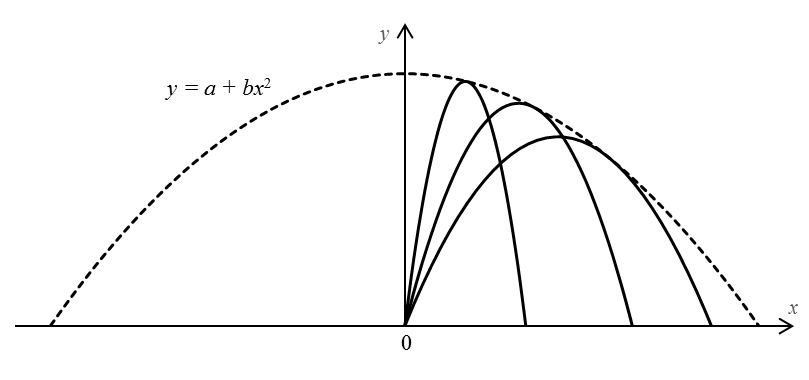
\includegraphics[width=\linewidth]{images/sjpo2016q11.png}
\end{wrapfigure}
\begin{itemize}
\item[](A) $\quad a=\frac{v_0{ }^2}{2 g}, b=\frac{g}{v_0{ }^2}$
\item[](B) $\quad a=\frac{v_0{ }^2}{2 g}, b=\frac{g}{2 v_0{ }^2}$
\item[](C) $\quad a=\frac{v_0{ }^2}{2 g}, b=\frac{2 g}{v_0{ }^2}$
\item[](D) $\quad a=\frac{v_0{ }^2}{g}, b=-\frac{g}{v_0{ }^2}$
\item[](E) $\quad a=\frac{v_0{ }^2}{2 g}, b=-\frac{g}{2 v_0{ }^2}$
\end{itemize}
Ans: \ifpaper E \fi \\[10pt]
Extra: Prove that the envelope is a parabola. \url{https://en.wikipedia.org/wiki/Envelope_(mathematics)}
\end{samepage}

\begin{samepage}
\subsubsection{SJPO 2014 General Round Q12: Projectile on Slope}
\url{https://youtu.be/l4lq6dXTug0}\\[10pt]
As shown in the figure below, a ball is thrown out horizontally from a slope. The slope makes an angle $\theta$ with the ground. At the first throw, the ball is ejected with a speed $v_1$ and at the second throw, it is ejected with a speed $v_2$. The angles that the ball made with the slope are measured to be $\alpha_1$ and $\alpha_2$ respectively. If $v_1$ is greater than $v_2$,\\
 \begin{wrapfigure}{r}{0.4\textwidth} 
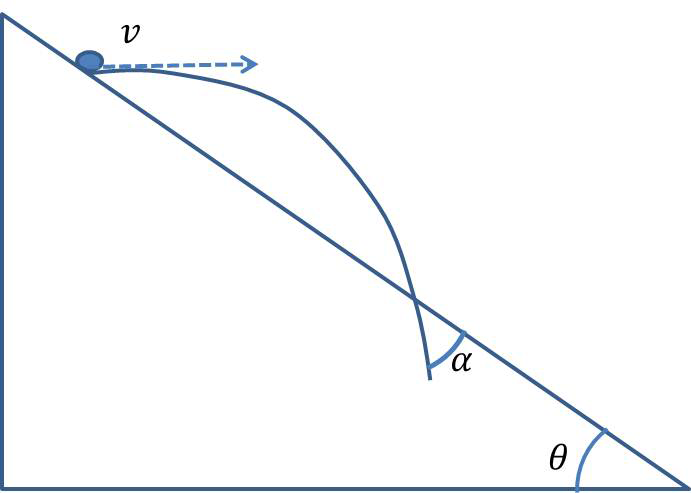
\includegraphics[width=\linewidth]{images/2014q12.png}
\end{wrapfigure}
\begin{itemize}
\item[](A) $\alpha_1=\alpha_2$
\item[](B) $\alpha_1>\alpha_2$
\item[](C) $\alpha_1<\alpha_2$
\item[](D) $\alpha<\theta$
\item[](E) It is not possible to infer much as the mass of the ball is not given.
\end{itemize}
Ans: \ifpaper A \fi \\[10pt]
\end{samepage}



% Hitting a slope\\
% Starting from a height \\
% Minimum velocity to cross a wall (spot)\\
% (ODE) With air resistance

\section{Physics: Constraining Forces}
Constraint forces are generally forces that will \textbf{adjust} their magnitude to \textbf{prevent some form of motion}. For example, normal contact force prevents objects from sinking into each other. Friction prevents rough objects from sliding with respect to each other. And tension in an inextensible string limits the distance between two objects. 
\subsection{Normal Contact Force}
Normal contact force $N$ between two rigid bodies \textbf{in contact} is a vector:
\begin{itemize}
    \item Direction: Always normal to the surfaces in contact, opposes "sinking"
    \item Magnitude: can range from $0$ to $\infty$. If magnitude is $0$, the two bodies is about to \textbf{lose contact}.
\end{itemize}
Normal contact force obeys N3L.
\subsection{Friction}
Frictional force between two rough bodies \textbf{in contact} is a vector: 
\begin{itemize}
    \item Direction: Always parallel to the surfaces in contact, opposes sliding
    \item Magnitude: can range from $|F_{\text{fric}}| \leq \mu_s N$. If friction is maxed out at $\mu_s N$, it will soon be unable to counteract the external forces, and the two bodies will \textbf{start sliding}.
\end{itemize}
$\mu_s$ is the static coefficient of friction. \\[10pt]
When sliding starts, the magnitude will be limited by the kinetic coefficient of friction $\mu_k$ instead of $\mu_s$. Usually $\mu_k < \mu_s$, which is why you will lose control of your car if your tyres skid.

\subsubsection{SJPO 2015 General Round Q12}
As shown in the figure below, the block with mass $M$ is stationary upon the plank and the angle of the slope $\theta$ is increased. Which of the following is true for the normal force of the block on the wooden plank, $N$ and the frictional force on the plank, $f$? \\
\begin{wrapfigure}{r}{0.36\textwidth}
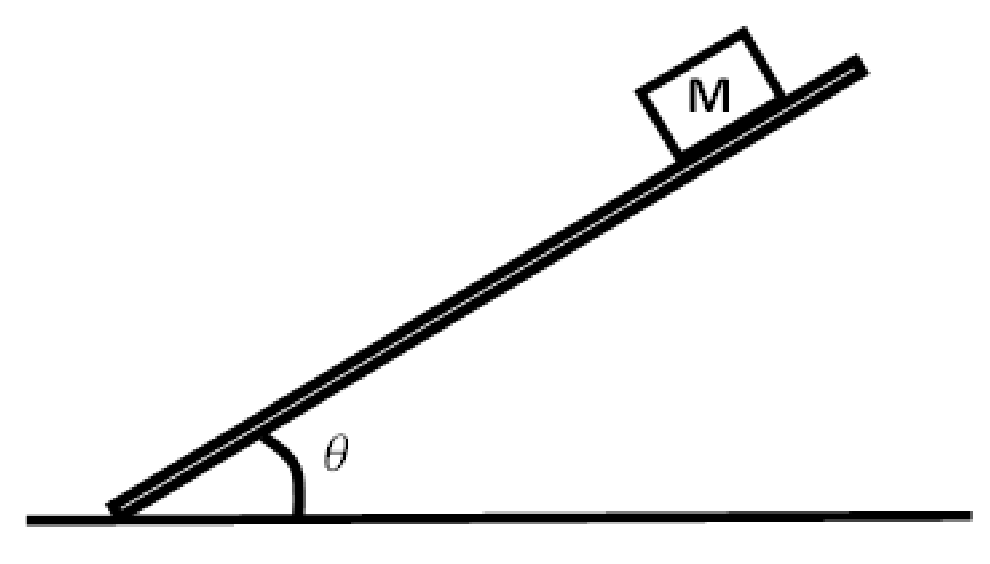
\includegraphics[width=1.0\linewidth]{images/sjpo2015q12.png}
\end{wrapfigure}


\begin{itemize}
\item[] (A) Both $N$ and $f$ increase.
\item[] (B) Both $N$ and $f$ decrease.
\item[] (C) $N$ increases and $f$ decreases.
\item[] (D) $N$ decreases and $f$ increases.
\item[] (E) The response differs when the value of $M$ is different.
\end{itemize}
Ans: \ifpaper D \fi \\[10pt]
Extra: If the static coefficient of friction is $\mu$, at what angle $\theta_{\text{max}}$ does the block begin slipping?



\subsubsection{SJPO 2016 General Round Q4}
A box is pulled using a string up a 0.1 radian slope at constant speed of $2.0 \mathrm{~ms}^{-1}$. The string is cut suddenly and the box comes to a stop after moving up a further distance of $1.0 \mathrm{~m}$. What is the value of the coefficient of friction?
{
\begin{wrapfigure}{r}{0.6\textwidth}
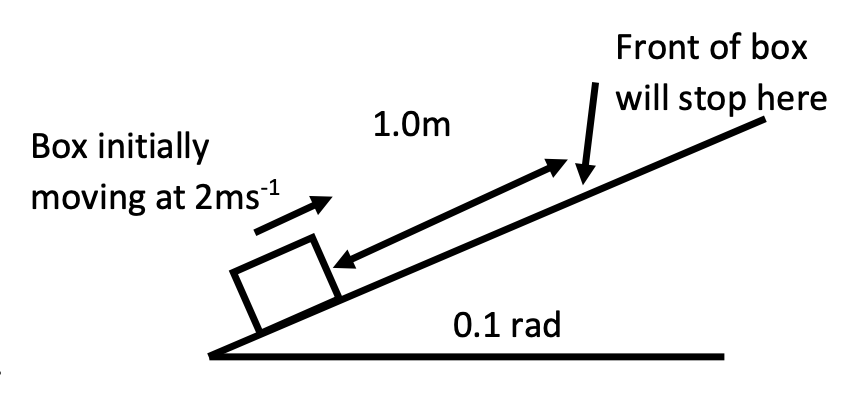
\includegraphics[width=1.0\linewidth]{images/sjpo2016q4.png}
\end{wrapfigure}
\begin{itemize}
\item[] (A) $\quad 0.00$
\item[] (B) $\quad 0.10$
\item[] (C) $\quad 0.20$
\item[] (D) $\quad 0.30$
\item[] (E) The situation is impossible.
\end{itemize}
}
Ans: \ifpaper B \fi
\subsection{Tension}
Tension in the string connecting two bodies is a vector:
\begin{itemize}
    \item Direction: \textbf{Isotropic} and constant anywhere \textbf{along the string}. Parallel and toward the string at \textbf{endpoints of string}.
    \item Magnitude: can range from $0$ to $\infty$, unless question specifies a limit. If the tension is $0$, the string is loose.
\end{itemize}
For a massless string (whether straight or curved on a pulley), tension is equal everywhere along the string (can be easily proven). This is particular useful for pulley questions. \\[10pt]
We will deal with massive string after talking about "mass distributions" (Topic of Moment of Inertia).\\[10pt]
Extra: A string on a pulley with friction has an exponential effect in increasing tension. See \url{https://en.wikipedia.org/wiki/Capstan_equation}. We will cover this in future too.

    
\subsubsection{SJPO 2018 General Round Q6}
\begin{wrapfigure}{r}{0.5\textwidth}
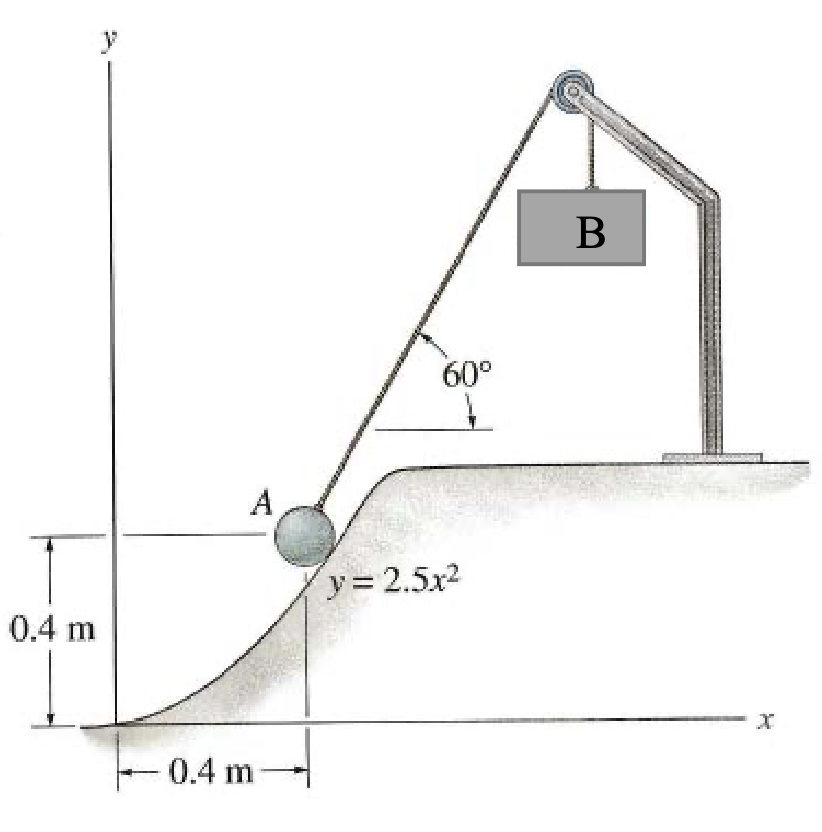
\includegraphics[width=1.0\linewidth]{images/sjpo2018q6.png}
\end{wrapfigure}
A $4 \mathrm{~kg}$ sphere rests on the smooth parabolic surface which is given by the equation $y=2.5 x^2$. The sphere just touches the surface at $(x, y)=(0.4 \mathrm{~m}, 0.4 \mathrm{~m})$. Determine the mass $m_{\mathrm{B}}$ of block B needed to hold the sphere in equilibrium.
\begin{itemize}
\item[] (A) $4.14 \mathrm{~kg}$
\item[] (B) $3.75 \mathrm{~kg}$
\item[] (C) $3.58 \mathrm{~kg}$
\item[] (D) $2.93 \mathrm{~kg}$
\item[] (E) $2.14 \mathrm{~kg}$
\end{itemize}
Ans: \ifpaper C \fi
\clearpage

\section{Physics: Drag / Air Resistance}

Drag is a force dependent on velocity and the \textbf{geometry} of the object.
\begin{align}
    F_{\text{drag}}(v) =\frac{1}{2} \rho v^2 C_D(v) A
\end{align}
\begin{itemize}
    \item $\rho$ is the density of the fluid
    \item $v$ is velocity of object relative to fluid
    \item $C_D(v)$ is dimensionless drag coefficient (usually obtained experimentally), which is a function of velocity
    \item $A$ is cross sectional area
\end{itemize}
At low velocities, $C_D(v) \propto 1/v$ approximately, so $F_{\text{drag}}(v) \propto v$ \\[10pt]
At high velocities, $C_D(v)$ is approximately constant, so $F_{\text{drag}}(v) \propto v^2$. \\[10pt]
In Physics Olympiad, the question will typically specify. \\[10pt]
Drag is the reason why falling objects have a terminal velocity
\subsection{Terminal Velocity}
(Taking the y-axis as downward positive), the net vertical forces on an object falling is
\begin{align}
    ma(t) = F_{\text{net}}(v) = mg - F_{\text{drag}}(v)
\end{align}
As $v(t)$ increases over time, drag force increases, causing $a(t)$ to decrease. The resultant motion is that $v(t)$ approaches asymptotically to a constant $v_{\text{terminal}}$, at which $$F_{\text{net}}(v_{\text{terminal}}) = 0$$

\subsection{Exercises}
\subsubsection{SJPO 2018 General Round Q2}
A tiny spherical raindrop of diameter $D=0.1 \mathrm{~mm}$ experiences a linear drag force while falling at speed $v$, given by $F_{\text {drag }}=c v$, where $c=1.55 \times 10^{-6} \mathrm{~N} \mathrm{~s} \mathrm{~m}^{-1}$. What is its terminal speed?
\begin{itemize}
\item[] (A) $1.7 \mathrm{~mm} / \mathrm{s}$
\item[] (B) $3.3 \mathrm{~mm} / \mathrm{s}$
\item[] (C) $8.5 \mathrm{~mm} / \mathrm{s}$
\item[] (D) $26 \mathrm{~mm} / \mathrm{s}$
\item[] (E) $33 \mathrm{~mm} / \mathrm{s}$
\end{itemize}
Ans: \ifpaper B \fi

\subsubsection{SJPO 2017 General Round Q7}
An object, \textbf{1}, with mass $m$ and another object, \textbf{2}, with twice the mass $2 m$ are dropped from rest, at the same starting position from the top of a large container and fall in a straight line through motionless viscous liquid. Drag is significant and assume that the two objects would eventually reach the same terminal velocity $v_T$ if the container were tall enough. Consider the case where the objects do not reach terminal velocity at the bottom of the container. Assume that the same type of drag acts on both objects. How does the time taken, $t_1$ and $t_2$, for the objects \textbf{1} and \textbf{2} to reach the bottom compare?\\[10pt]
{
 \begin{wrapfigure}{r}{0.5\textwidth} 
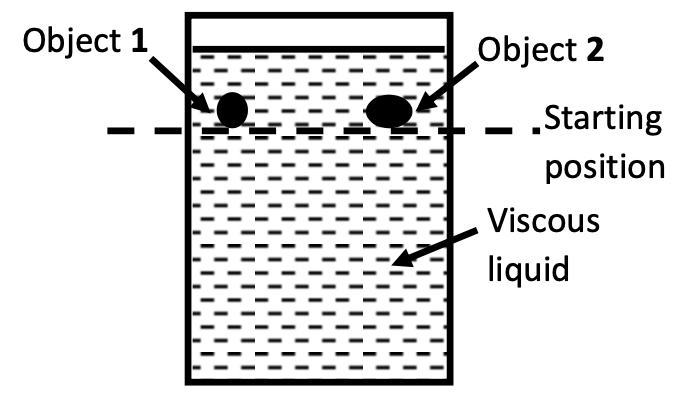
\includegraphics[width=\linewidth]{images/sjpo2016q7.png}
\end{wrapfigure}
\begin{itemize}
\item[] (A) $t_1=t_2$
\item[] (B) $t_1<t_2$
\item[] (C) $t_1>t_2$
\item[] (D) $t_2<t_1<2 t_2$
\item[] (E) $t_1<t_2<2 t_1$
\end{itemize}
}
Ans: \ifpaper A \fi


\subsection{Extra: Up and Down with Air Resistance}
In a case \textbf{without air resistance}, if we throw a ball up, suppose it takes $T_1$ seconds to reach the peak from the time it was released, and $T_2$ seconds to fall back down from the peak to the original point of release. One can prove $T_1 = T_2$ easily.\\[10pt]
In a case \textbf{with air resistance},
suppose the time to reach the peak is $\tau_1$ and the time to drop down is $\tau_2$. \textbf{Prove rigorously} that $\tau_1 < \tau_2$.\\[10pt]
\url{https://youtu.be/1uaHkc3TfBU}

\subsection{Extra: Projectile Motion with Drag}
It is possible to solve for projectile motion exactly, but only after we study differential equations. We postpone this to the future.

\section{Physics: Collisions}
Collisions between multiple bodies (e.g. dropping a stack of balls) are analysed as a sequence of collisions between 2 bodies at a time. When 2 bodies collide, their \textbf{total momentum is always conserved} / invariant before and after the collision (invariant means doesn't change). Their total energy, however, has 3 possibilities:
\begin{itemize}
    \item Total energy conserved (\textbf{elastic})
    \item Total energy decreased (\textbf{inelastic}) e.g. billiard balls
    \item Total energy increased (\textbf{superelastic}) e.g. compressed spring, explosion
\end{itemize}
\subsection{Momentum Conservation}
\textbf{Q}: Why is momentum invariant before and after the collision? \\[10pt]
\textbf{A}: Momentum conservation is due to Newton's 3rd Law. To see this, recall that an object's momentum changes by impulse 
$$\Delta \vec{p} \text{ from } t_0 \text{ to } t_1 = \int_{t_0}^{t_1} \vec{F}(t)\ dt$$
By Newton's 3rd Law, when 2 bodies interact, the forces they exert on each other are equal in magnitude and opposite in direction. 
$$\vec{F}_{\text{A on B}} = -\vec{F}_{\text{B on A}}$$
Integrating both sides wrt time $t$, one sees that the impulse they experience is also equal in magnitude and opposite in direction.
$$\Delta \vec{p}_B = - \Delta \vec{p}_A$$
As such, the sum of their momentum remains unchanged.
$$\Delta(\vec{p}_A + \vec{p}_B) = \vec{0}$$
This remains true for all forces that obey N3L, including collisions (normal contact force). 
\subsection{1D Elastic Collisions}
Let the masses be $m_A, m_B$, the initial velocities be $u_A, u_B$ and final velocities be $v_A, v_B$. Conservation of momentum and energies yields
\begin{align}
    m_A u_A + m_B u_B &= m_A v_A + m_B v_B \\
    \frac{1}{2} m_A u_A^2 + \frac{1}{2} m_B u_B^2 &= \frac{1}{2} m_A v_A^2 + \frac{1}{2} m_B v_B^2 
\end{align}
Rearranging both equations gives us (respectively)
\begin{align}
    m_A (u_A - v_A) &= - m_B (u_B - v_B) \label{eq:com}\\
    m_A (u_A - v_A) (u_A + v_A) &= - m_B (u_B - v_B) (u_B + v_B) \label{eq:coe}
\end{align}
If we divide equation \ref{eq:coe} by \ref{eq:com} we obtain
\begin{align}
    u_A + v_A &= u_B + v_B \\
    \Rightarrow u_A - u_B &= - (v_A - v_B)
\end{align}
\begin{samepage}
This equation is sometimes said verbally as 
\begin{center}
    \textbf{velocity of approach = velocity of separation}
\end{center}
\end{samepage}
This is because if object A is positioned to the left of object B (and our choice of axis direction is rightward positive), then a positive $u_A - u_B > 0$ would imply that A is getting closer to B, and $u_A - u_B$ describes how fast the distance between them is decreasing. Hence, $u_A - u_B > 0$ is called the \textbf{velocity of approach}. \\[10pt]
After the collision, $v_A - v_B = -(u_A - u_B) < 0$ implies that B is getting further and further away from A. $-(v_A - v_B) > 0$ quantifies how fast the distance between them is increasing. Hence, $-(v_A - v_B) > 0$ is called the \textbf{velocity of separation}.\\[10pt]
Anyway, previously we had one linear equation (momentum) and one quadratic equation (energy). Now we have 2 linear equations (momentum and "rate of approach = separation")
\begin{align}
    m_A u_A + m_B u_B &= m_A v_A + m_B v_B \label{eq:com2}\\
    u_A - u_B &= - (v_A - v_B) \label{eq:voaevos}
\end{align}
Linear simultaneous equations are easy to solve, rearrange equation (\ref{eq:voaevos}) and substitute $v_A = v_B - u_A + u_B$ into (\ref{eq:com2}) to obtain
\begin{align}
    m_A u_A + m_B u_B &= m_A (v_B - u_A + u_B) + m_B v_B \\
    &= (m_A + m_B) v_B - m_A u_A + m_A u_B \\
    v_B &= \frac{2m_A}{m_A + m_B} u_A + \frac{m_B - m_A}{m_A + m_B} u_B 
\end{align}
Repeating this with $v_B = u_A - u_B + v_A$ gives us 
\begin{align}
    m_A u_A + m_B u_B &= m_A v_A + m_B (u_A - u_B + v_A) \\
    &= (m_A + m_B) v_A + m_B u_A - m_B u_B \\
    v_A &= \frac{m_A - m_B}{m_A + m_B} u_A + \frac{2m_B}{m_A + m_B} u_B
\end{align}
One sees that the final velocities almost look like they have a nice symmetry to them. You can memorise these formulas but personally I just derive it every time I need it because I don't like memorising.
\subsubsection{SJPO 2017 General Round Q40}
40. A small tennis ball with mass $m$ sits atop a large basketball with mass $M$, with $M \gg m$. The balls are released from rest, with the bottom of the basketball at a height $\mathrm{h}$ above the ground. The diameter of the tennis ball is d and that of the basketball is $D$, with $D \gg d \approx 0$. To what height does the tennis ball bounce above the ground? Assume all collisions are elastic.
\begin{itemize}
\item[] (A) $D+h$
\item[] (B) $D+4 h$
\item[] (C) $D+8 h$
\item[] (D) $D+9 h$
\item[] (E) There is insufficient information.
\end{itemize}
Ans: \ifpaper D \fi
Extra: There is an extension of this to multiple balls in H3 physics \url{https://youtu.be/drVTrXib-7g?t=260}

\subsection{Center of Momentum Frame}
The Center of Momentum frame (CoM) is very useful because it simplifies the momentum equation greatly. The CoM frame is defined to be the frame in which the total momentum is zero. So, in any dimension,
\begin{align}
    m_A \mathbf{u}_{A,CM} + m_B \mathbf{u}_{B,CM} &= m_A \mathbf{v}_{A,CM} + m_B \mathbf{v}_{B,CM} = \mathbf{0} \label{eq:zeromomentum}
\end{align}
where the bolded quantities $\mathbf{u}$ emphasise that this is a vector equation. We can show that such a frame exists by proof by construction 
\begin{align}
    \mathbf{u}_A &\equiv \mathbf{u}_{CM} + \mathbf{u}_{A,CM} \\
    \mathbf{u}_B &\equiv \mathbf{u}_{CM} + \mathbf{u}_{B,CM} \\
    \text{Define/Choose }\mathbf{u}_{CM} &= \frac{m_A \mathbf{u}_A + m_B \mathbf{u}_B}{m_A + m_B} \\
    m_A \mathbf{u}_{A,CM} + m_B \mathbf{u}_{B,CM} &= m_A (\mathbf{u}_A  - \mathbf{u}_{CM}) + m_B (\mathbf{u}_B - \mathbf{u}_{CM}) \\
    &= m_A \mathbf{u}_A + m_B \mathbf{u}_B - (m_A + m_B) \mathbf{u}_{CM} \\
    &= \mathbf{0}
\end{align}
Rearranging the zero total momentum equation (\ref{eq:zeromomentum}) yields A's velocities in terms of B's velocities
\begin{align}
    \mathbf{u}_{A,CM} &= -\frac{m_B}{m_A} \mathbf{u}_{B,CM} \\
    \mathbf{v}_{A,CM} &= -\frac{m_B}{m_A} \mathbf{v}_{B,CM} 
\end{align}
which can be substituted into the conservation of energy equation to eliminate A's initial and final velocities, leaving us with an equation purely relating B's initial and final velocities
\begin{align}
    \frac{1}{2} m_A \mathbf{u}_{A}^2 + \frac{1}{2} m_B \mathbf{u}_{B}^2  &= \frac{1}{2} m_A \mathbf{v}_{A}^2 + \frac{1}{2} m_B \mathbf{v}_{B}^2 \\
    \Rightarrow \left( \frac{m_B^2}{m_A} + m_B \right) \mathbf{u}_{B,CM}^2 &= \left( \frac{m_B^2}{m_A} + m_B \right) \mathbf{v}_{B,CM}^2 \\
    \Rightarrow \mathbf{u}_{B,CM}^2 &= \mathbf{v}_{B,CM}^2 
\end{align}
\subsubsection{1D Elastic Collision Revisited using CoM Frame}
The CoM equations become
\begin{align}
    m_A u_{A,CM} + m_B u_{B,CM} &= 0 \\
    m_A v_{A,CM} + m_B v_{B,CM} &= 0 \\
    u_{B,CM}^2 &= v_{B,CM}^2 
\end{align}
If B is to the right of A (and our axis is defined as rightward positive), then $u_{B,CM} < 0$ because B is moving left in the CM frame before the collision. $v_{B,CM} > 0$ because B is moving right in the CM frame after the collision. Hence 
\begin{align}
    u_{B,CM}^2 &= v_{B,CM}^2 \\
    \Rightarrow v_{B,CM} &= -u_{B,CM} \\
    v_{A,CM} &= -\frac{m_B}{m_A} v_{B,CM} \\ 
    &= \frac{m_B}{m_A} u_{B,CM} \\
    &= - u_{A,CM}
\end{align}
Wow! What a remarkably neat result. In the CoM frame, the velocities simply flip direction during the collision. Returning to the lab frame, we obtain 
\begin{align}
    v_A &= u_{CM} + v_{A,CM} \\
    &= u_{CM} - u_{A,CM} \\
    &= u_{CM} - (u_A - u_{CM}) \\
    &= 2 u_{CM} - u_A \\
    &= 2 \frac{m_A u_A + m_B u_B}{m_A + m_B} - u_A\\
    v_A &= \frac{m_A - m_B}{m_A + m_B} u_A + \frac{2m_B}{m_A + m_B} u_B \\
    v_B &= \frac{2m_A}{m_A + m_B} u_A + \frac{m_B - m_A}{m_A + m_B} u_B
\end{align}
which matches our 1D elastic collision result. Calculation wise, one might not see the merits of CoM frame in 1D. But intuition wise, the fact that the velocities just flip during the collision gives us the intuition that the balls are just hitting an imaginary wall at the point of collision. \\[10pt]
The real power of CoM frame comes in when we consider 2D or 3D collisions. The intuition of the objects hitting a wall still holds true, but in 2D the wall is slanted at an angle. We discuss more about this now.
\subsection{2D Elastic Collisions}
In 2D elastic collisions, there are 4 unknowns $v_{A,x}, v_{A,y}, v_{B,x}, v_{B,y}$ but only 3 equations from momentum and energy conservation.
\begin{align}
m_A u_{A,x} + m_B u_{B,x} &= m_A v_{A,x} + m_B v_{B,x} \\
m_A u_{A,y} + m_B u_{B,y} &= m_A v_{A,y} + m_B v_{B,y} \\
    \frac{1}{2} m_A (u_{A,x}^2 + u_{A,y}^2) + \frac{1}{2} m_B (u_{B,x}^2 + u_{B,y}^2) 
 &= \frac{1}{2} m_A (v_{A,x}^2 + v_{A,y}^2) + \frac{1}{2} m_B (v_{B,x}^2 + v_{B,y}^2) 
\end{align}
We need 4 equations, but the 4th equation cannot be determined from physics alone. It is a parameter we need to put in by hand, and this parameter can be any (non-trivial) relation between the velocities. An example would be the final angle of velocity of A $\vec{v}_{A}$
\begin{align}
    v_{A,y} = v_{A,x} \tan \theta_A
\end{align}
but really any other constraint could do. Solving these 4 simultaneous equations is possible but extremely tedious. Therefore, it will help alot to consider the CoM frame. From the previous section, we derived the following result
\begin{align}
    \mathbf{u}_{A,CM}^2 &= \mathbf{v}_{A,CM}^2 \\ 
    \mathbf{u}_{B,CM}^2 &= \mathbf{v}_{B,CM}^2 \\ 
    \mathbf{u}_{A,CM} &= -\frac{m_B}{m_A} \mathbf{u}_{B,CM}\\
    \mathbf{v}_{A,CM} &= -\frac{m_B}{m_A} \mathbf{v}_{B,CM}
\end{align}
In the CoM frame, both objects are bouncing off an imaginary common wall elastically. Conservation of momentum and energy doesn't dictate what the angle of the wall is, we need to specify so by a parameter $\theta$. \\[10pt]
Extra: This extends to 3D as well! But this time the wall is a 2D plane, and the normal vector of the wall is described by 2 angles $\theta,\phi$.\\[10pt]
\subsubsection{SJPO 2017 General Round Q42: Max Deflection}
A mass $M$, with initial speed $V$, collides elastically with a stationary mass $m=M / 2$. Find the maximum angle of deflection of the mass $M$.
\begin{itemize}
\item[] (A) $180^{\circ}$
\item[] (B) $120^{\circ}$
\item[] (C) $30^{\circ}$
\item[] (D) 0
\item[] (E) There is insufficient information to tell.
\end{itemize}
Ans: \ifpaper C \fi
% In most physics questions, however, we aren't required to solve the general case. Sometimes the CoM frame isn't necessary. Typically these questions are just a test of your simultaneous equation solving skills (that's really most mechanics questions anyway).
\subsection{1D Inelastic Collisions}
Conservation of momentum still holds, but some energy is lost in the form of heat and sound. Instead of having an equation from energy, we parameterize the inelastic collision with \textbf{coefficient of restitution} $0\leq e \leq 1$, defined by the ratio of the velocity of separation over the velocity of approach, which is information that needs to be provided by the question. The 2 linear equations are 
\begin{align}
    m_A u_A + m_B u_B &= m_A v_A + m_B v_B \\
    e (u_A - u_B) &= -(v_A - v_B)
\end{align}
Solving these 2 simultaneously gives us
\begin{align}
    v_A &= \frac{e m_B (u_B - u_A) + m_A u_A + m_B u_B}{m_A + m_B} \\
    v_B &= \frac{e m_A (u_A - u_B) + m_A u_A + m_B u_B}{m_A + m_B}
\end{align}
One can see that substituting $e=1$ recovers the result for elastic collision. In fact, one can kind of see that these equations are even easier to memorize than the elastic ones. 
\subsubsection{SJPO 2018 General Round Q14}
Two blocks move towards each other on a smooth table with the velocities as shown. Block A has mass $5 \mathrm{~kg}$ and moves at $2 \mathrm{~m} / \mathrm{s}$ to the right. Block B has mass $2 \mathrm{~kg}$ and moves at $5 \mathrm{~m} / \mathrm{s}$ to the left. The coefficient of restitution $e$ is the ratio of the final relative speed of separation to the initial relative speed of approach of two colliding objects. Take rightwards as positive. If $e=0.5$, what is the velocity of block B after impact?
\begin{itemize}
\item[] (A) $-2.5 \mathrm{~m} / \mathrm{s}$
\item[] (B) $-1.0 \mathrm{~m} / \mathrm{s}$
\item[] (C) $0 \mathrm{~m} / \mathrm{s}$
\item[] (D) $ 1.0 \mathrm{~m} / \mathrm{s}$
\item[] (E) $ 2.5 \mathrm{~m} / \mathrm{s}$
\end{itemize}
Ans: \ifpaper E \fi
\subsection{1D Perfectly Inelastic}
Perfectly inelastic collisions are inelastic collisions where $e=0$. This implies that $v_A = v_B$, which physically means that the 2 bodies stick together after the collision and effectively travel as one. \\[10pt]
\textbf{Maximum Kinetic Energy Loss} occurs in inelastic collisions. One can see this clearly in the CoM frame, where both objects collide with each other and stop moving. 
\subsubsection{SJPO 2017 General Round Q49}
A long, hard train collides with a small fly. Assume the mass of the fly is negligible compared to the mass of the train. The train and the fly were initially moving towards each other with the same magnitude of velocity. When they collide, the train and fly stick to each other and finally travel with the same velocity as each other. Which of the following statements is most true in relation to the above?
\begin{itemize}
\item[] (A) During the collision the velocity of the fly changes direction instantaneously to that of the train.
\item[] (B) During the collision the fly stops moving at some point in time since the velocity changes in direction.
\item[] (C) Since the velocity of the fly must be zero at some time during the collision and it is attached to the train, then the train also has zero velocity at that time.
\item[] (D) After the collision the fly must have gained momentum from the train.
\item[] (E) The train must have exerted a large force on the fly due to its large momentum. The force exerted on the fly is proportional to the momentum of the train.
\end{itemize}
Ans: \ifpaper B \fi
\subsubsection{SJPO 2016 General Round Q24}
Case 1: A $80 \mathrm{~kg}$ skater with speed $u$ slides towards stationary skater with mass $20 \mathrm{~kg}$. They \textbf{hold hands} when they reach each other and continue as one. \\[10pt]
Case 2: the $20 \mathrm{~kg}$ skater is moving and the 80 kg skater is stationary; the initial kinetic energy of the systems in both cases are the same. \\[10pt]
Assume friction is negligible. What is the ratio of the \textbf{change in kinetic energy} (i.e the amount of energy converted to other forms) of the system in case 1 to that in case 2? i.e. (case 1 : case 2)
\begin{itemize}
\item[] (A) $4: 1$
\item[] (B) $2: 1$
\item[] (C) $1: 1$
\item[] (D) $1: 2$
\item[] (E) $1: 4$
\end{itemize}
Ans: \ifpaper E \fi
\subsection{Accounting for Rotation}
So far the objects were assumed to be point masses, or solid bodies that only move translationally. In reality we know objects can rotate before and after the collision. Rotational dynamics is what we will cover now.
\clearpage
\section{Physics: Assorted Practice}

\subsubsection{SJPO 2016 General Round Q1}
A force is applied to a box to push it across the horizontal floor at a constant speed of $4.0 \mathrm{~m} / \mathrm{s}$. Assume air resistance is negligible. What can you say about the forces acting on the box?
\begin{itemize}
\item[] (A) If the force applied to the box is doubled, the constant speed of the box will double to $8.0 \mathrm{~m} / \mathrm{s}$.
\item[] (B) The magnitude of force applied to keep the box moving at a constant speed must be more than the magnitude of its weight.
\item[] (C) The force being applied to the box to keep it moving at constant speed makes an action-reaction pair with the frictional force that resists its motion.
\item[] (D) The magnitude of force applied to keep the box moving at a constant speed must be equal to the magnitude of the frictional forces that resist its motion.
\item[] (E) The magnitude of force applied to keep the box moving at a constant speed must overcome i.e. be more than the magnitude of the frictional forces that resist its motion.
\end{itemize}
Ans: \ifpaper D \fi

\subsubsection{SJPO 2016 General Round Q2}
If the force applied to the box in the preceding problem is suddenly discontinued, the box will
\begin{itemize}
\item[] (A) stop suddenly.
\item[] (B) continue at a constant velocity.
\item[] (C) suddenly start slowing to a stop.
\item[] (D) increase its speed for a very short period of time, then start slowing to a stop.
\item[] (E) continue at a constant speed for a very short period of time and then slow to a stop.
\end{itemize}
Ans: \ifpaper C \fi


\subsubsection{SJPO 2016 General Round Q6}
Carts $\mathrm{A}$ and $\mathrm{B}$ are initially at rest on a frictionless, horizontal surface. A constant force $F_0$ is applied to each cart as it travels from its initial position. The mass of cart $\mathbf{A}$ is more than the mass of cart $\mathbf{B}$. Consider the kinetic energy, $E$, and momentum, $p$, of the boxes at position $\mathrm{X}$, a distance $x_0$ from the initial position. Subscripts A, B denote cart A or B. Which statement below is correct?
{
\begin{wrapfigure}{r}{0.5\textwidth}
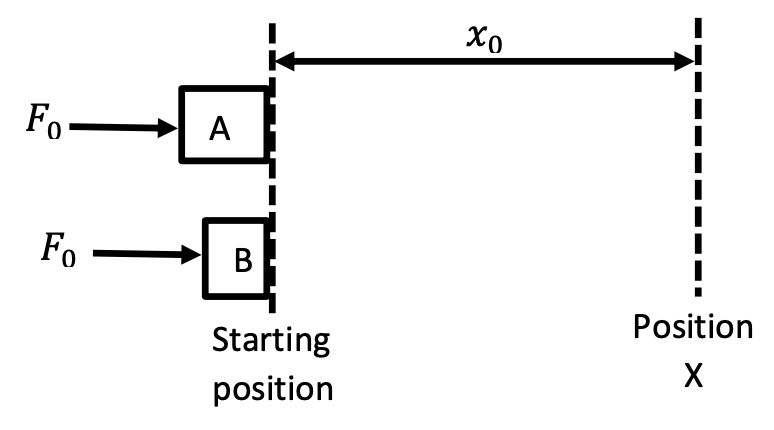
\includegraphics[width=1.0\linewidth]{images/sjpo2016q6.png}
\end{wrapfigure}
\begin{itemize}
\item[] (A) $E_A<E_B, p_A<p_B$
\item[] (B) $E_A<E_B, p_A=p_B$
\item[] (C) $E_A>E_B, p_A<p_B$
\item[] (D) $E_A=E_B, p_A=p_B$
\item[] (E) $E_A=E_B, p_A>p_B$
\end{itemize}
}
Ans: \ifpaper E \fi


\subsubsection{SJPO 2016 General Round Q12}
The upper end of a rope is fixed to a vertical wall. The upper end makes an angle of 30 degrees with the wall when the lower end is pulled by a horizontal force of $20 \mathrm{~N}$. What is the mass of the rope?
{
\begin{wrapfigure}{r}{0.5\textwidth}
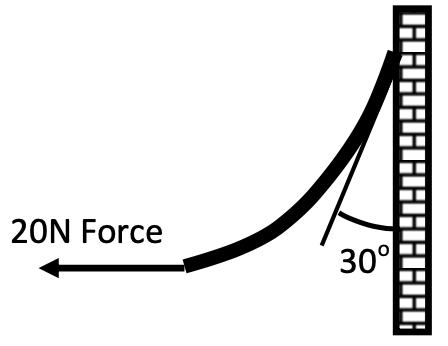
\includegraphics[width=1.0\linewidth]{images/sjpo2016q12.png}
\end{wrapfigure}
\begin{itemize}
\item[] (A) $1.8 \mathrm{~kg}$
\item[] (B) $2.0 \mathrm{~kg}$
\item[] (C) $2.4 \mathrm{~kg}$
\item[] (D) $3.5 \mathrm{~kg}$
\item[] (E) $4.1 \mathrm{~kg}$
\end{itemize}
}
Ans: \ifpaper D \fi

\subsubsection{SJPO 2018 General Round Q11}
% SJPO 2018 General Round Q11 B
The minimum time $T$ for a car to safely overtake a long trailer is measured from the time the front of the car is level with the rear of the trailer, until the rear of the car is one full car-length ahead of the trailer. The car is $3.5 \mathrm{~m}$ long and the trailer is $15.0 \mathrm{~m}$ long.\\[10pt]
The graph shows the speed-time graphs of the car and the trailer. What is the minimum time $T$ ?\\
{
\begin{wrapfigure}{r}{0.5\textwidth}
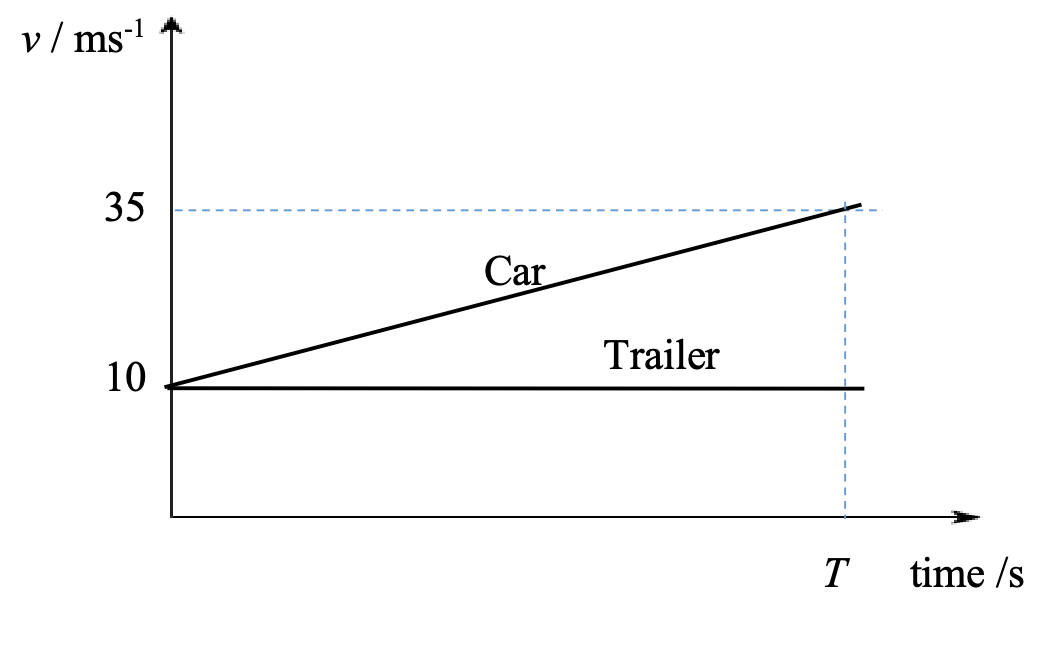
\includegraphics[width=1.0\linewidth]{images/sjpo2018q11.png}
\end{wrapfigure}
\begin{itemize}
\item[] (A) $\quad 2.16 \mathrm{~s}$
\item[] (B) $\quad 1.76 \mathrm{~s}$
\item[] (C) $\quad 1.48 \mathrm{~s}$
\item[] (D) $\quad 0.88 \mathrm{~s}$
\item[] (E) $\quad 0.64 \mathrm{~s}$
\end{itemize}
Ans: \ifpaper B \fi
}
\subsubsection{SJPO 2018 General Round Q12}
{
\begin{wrapfigure}{r}{0.4\textwidth}
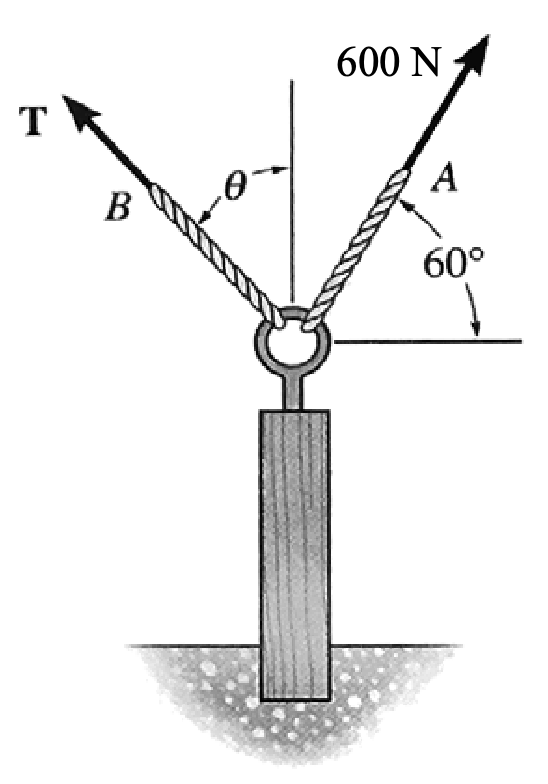
\includegraphics[width=1.0\linewidth]{images/sjpo2018q12.png}
\end{wrapfigure}
A wooden peg is to be pulled out of the ground using two ropes A and B. Rope $\mathrm{A}$ is subject to a force of $600 \mathrm{~N}$ at $60^{\circ}$ to the horizontal. Rope $\mathrm{B}$ is pulled at a fixed angle $\theta$ to the vertical. If the resultant force acting on the post is to be $1600 \mathrm{~N}$ vertically, what should be the force $T$ on rope B?
\begin{itemize}
\item[] (A) $1121 \mathrm{~N}$
\item[] (B) $1334 \mathrm{~N}$
\item[] (C) $1400 \mathrm{~N}$
\item[] (D) $1924 \mathrm{~N}$
\item[] (E) $2040 \mathrm{~N}$
\end{itemize}
Ans: \ifpaper A \fi
}

\subsubsection{SJPO 2018 General Round Q13}
Travelling with an initial speed of $70 \mathrm{~km} / \mathrm{h}$, a car accelerates at $6000 \mathrm{~km} / \mathrm{h}^2$ along a straight road. How long will it take to reach a speed of $120 \mathrm{~km} / \mathrm{h}$ ?
\begin{itemize}
\item[] (A) $30 \mathrm{~s}$
\item[] (B) $45 \mathrm{~s}$
\item[] (C) $60 \mathrm{~s}$
\item[] (D) $70 \mathrm{~s}$
\item[] (E) $180 \mathrm{~s}$
\end{itemize}
Ans: \ifpaper A \fi

\begin{samepage}
\subsubsection{SJPO 2018 General Round Q18}
A $2 \mathrm{~kg}$ block slides down a smooth roof which is angled at $30^{\circ}$ to the horizontal. When it reaches $\mathrm{A}$, it has a speed of $2.0 \mathrm{~m} / \mathrm{s}$. It leaves the surface of the roof at $\mathrm{B}$ and strikes the ground at a distance $d$ from the wall of the building. What is the distance $d$ ?
{
 \begin{wrapfigure}{r}{0.4\textwidth} 
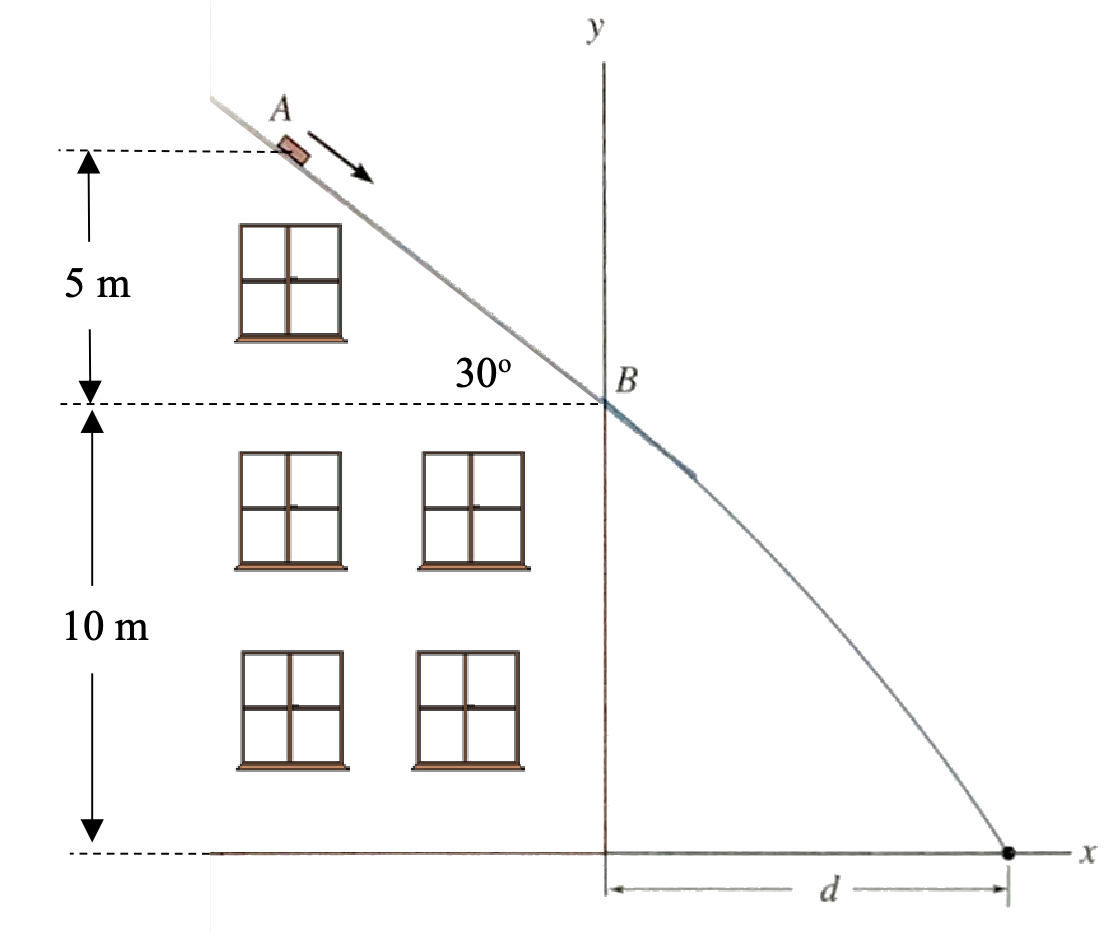
\includegraphics[width=\linewidth]{images/2018q18.png}
\end{wrapfigure}
\begin{itemize}
\item[](A) $3.96 \mathrm{~m}$
\item[](B) $8.66 \mathrm{~m}$
\item[](C) $8.78 \mathrm{~m}$
\item[](D) $17.3 \mathrm{~m}$
\item[](E) $17.8 \mathrm{~m}$
\end{itemize}
}
Ans: \ifpaper C \fi \\[10pt]
\end{samepage}



\section{Physics: Work and Impulse}

\subsubsection{SJPO 2016 General Round Q5}
A train of mass $7.0 \times 10^4 \mathrm{~kg}$ expends $60 \mathrm{~kW}$ of power to travel down a $2^{\circ}$ incline at a constant velocity of $10 \mathrm{~m} \mathrm{~s}^{-1}$. How much power is required for the same train to travel up the $2^{\circ}$ incline at the same constant velocity of $10 \mathrm{~m} \mathrm{~s}^{-1}$ ?
\begin{itemize}
\item[] (A) $540 \mathrm{~kW}$
\item[] (B) $480 \mathrm{~kW}$
\item[] (C) $300 \mathrm{~kW}$
\item[] (D) $240 \mathrm{~kW}$
\item[] (E) $60 \mathrm{~kW}$
\end{itemize}
Ans:  \ifpaper A \fi
\section{Math: Differential Equations}
When we studied $F(t)=ma(t)$, we noted that as long as we know the function $F(t)$, we can find $a(t)$ and integrate twice to obtain $x(t)$. However, in most systems, $F(t)$ depends on $x(t)$ or $v(t) \equiv \dot{x}(t)$. Examples include 
\begin{itemize}
    \item Spring Mass $F(x(t)) = -kx(t)$
    \item Gravitation $F(\vec{r}(t)) = -\frac{GMm}{|\vec{r}(t)|^2} \hat{r}$
    \item Drag $F(v(t)) = \frac{1}{2} \rho v(t)^2 C_D A$
    \item Lorentz Force $\vec{F} = q(\vec{E} + \vec{v} \times \vec{B})$
\end{itemize}
In these scenarios, we can no longer simply "integrate twice" since we hit a circular dependency. To resolve this, we need to solve the "differential equation". Differential equations are very common in physics. If you solve the Navier-Stokes Differential Equation, you earn a million dollars.

\subsection{What is a Differential Equation?}
When we first learned the quadratic equation, we were looking for \textbf{values} of $x$ that satisfy $$ax^2 + bx + c = 0$$  We can find 2 complex \textbf{solutions} to this \textbf{algebraic} equation
$$x = \frac{-b - \sqrt{b^2 - 4ac}}{2a} \quad \text{or}\quad x = \frac{-b + \sqrt{b^2 - 4ac}}{2a}$$
In \textbf{differential} equations, we are looking for \textbf{functions} $y(x)$ that satisfy (for example)
$$\frac{dy}{dx} = y$$
In this example, $y(x) = e^x$ works! Substitute it into the above to check that $\text{LHS} = \text{RHS}$. In fact, one can check that any multiple of $e^x$ works too! So $y(x) = A e^x$ for any arbitrary constant $A$ is a solution. To determine $A$, we need to know the "initial condition" $y(0) = A$.
\\[10pt]
Let's try another example, find the function $y(x)$ that satisfies 
$$\frac{dy}{dx} = 5y$$ with initial condition $\left. \frac{dy}{dx} \right|_{x=0} = 10$\\
Solution: $y(x) = 2e^{5x}$
\subsubsection{Physics: RC circuit} 
Find $q(t)$ that satisfies the following ($R,C$ are constants).
$$\frac{dq}{dt} = -\frac{q}{RC}$$ with initial condition $q(t=0) = q_0$. \\Answer: $q(t) = q_0 \exp (-t/RC)$ \\[10pt]
What if the initial condition was $I(t=0) := \left. \frac{dq}{dt} \right|_{t=0} = I_0$ instead? \\ Answer: $q(t) = {I_0 RC} \exp (-t/RC)$\\[10pt]

\subsection{Simple Harmonic Motion ODE}
In polynomial equations, the largest power $x^n$ is the degree $n$ of the polynomial. In differential equations, the highest derivative $\frac{d^n y}{dx^n}$ is the order of the differential equation. In this section, we cover a very common class of 2nd order differential equations
$$\frac{d^2 y}{dx^2} = -\omega^2 y$$
which has solution
$$y(x) = A\sin(\omega x + \phi)$$
\subsubsection{Derivation by Layman Arguments}
$\sin x$ and $\cos x$ are the only (proof involves linear algebra) functions that when differentiated twice, pick up a negative sign. We can afford to put a constant $\phi$ in the parameter of $\sin$, since constants vanish when differentiated. 

\subsubsection{Derivation using Complex Exponential }
\begin{align}
    \frac{d^2 y}{ dx^2} = A y     \label{eq:shm}
\end{align}
where $-\infty < A < \infty$ is a real constant.\\[10pt]
Solution: $$y=y_0 \exp(\sqrt{A}x)$$ 
Question: What happens if $A < 0$? \\
Answer: $\sqrt{A}$ is complex! To be more precise, if $A=-\omega^2$ for a positive real number $\omega$, then 
$$y=y_0 \exp(\pm i \omega x)$$
are 2 valid solutions.\\[10pt]
\textbf{A word on linear differential equation: } Equation \ref{eq:shm} is said to be linear, because if I have 2 solutions $f(x)$ and $g(x)$, then adding them together or scaling them is still a valid solution.
\begin{align}
    \text{Given } \frac{d^2 f}{ dx^2} &= A f(x)\\
    \text{And } \frac{d^2 g}{ dx^2} &= A g(x) \\
    y(x) &= f(x) + g(x)\text{ is a solution too }\\
    \text{Goal: Show } \frac{d^2y}{dx^2} & = Ay(x)\\
    \text{Proof: LHS} &= \frac{d^2}{dx^2} [f(x)+g(x)] \\
    &= \frac{d^2 f}{dx^2} + \frac{d^2 g}{dx^2} \\ 
    &= A f(x) + A g(x) \\
    &= A [f(x) + g(x)] \\
    &= \text{RHS}
\end{align}
Examples of Linear Differential Equations:
\begin{itemize}
    \item Simple Harmonic Motion
    \item RLC Circuits (linear components)
    \item (Linear) Wave Equation
    \item Schrodinger equation (Quantum Mechanics)
    \item Maxwell's Equation (Electromagnetism)
\end{itemize}
\leavevmode \\
Since $$y_+(x)=y_0 \exp(+ i \omega x)$$  $$y_-(x) = y_0 \exp(- i \omega x)$$ are 2 solutions to the \textbf{linear} DE $$\frac{d^2 f}{ dx^2} = A f(x)$$
any linear combination of them is a valid solution.

$$y(x) = C \exp(+i\omega x) + D \exp(-i \omega x)$$
where $C,D$ are arbitrary complex constants.\\[10pt]
\textbf{But what is a complex exponential? } Euler's formula: 
$$e^{i\theta} = \cos \theta + i \sin \theta$$
Some say it's just a mathematical trick, since "our system doesn't involve complex numbers". It gets philosophical. Richard Feynman famously said: "Shut up and calculate". \\[10pt]
So we want our solution $y(x)$ to be real, i.e. $\text{Im }[y(x)] = 0$. So that necessitates that $C^* = D$ and so the general solution is 
\begin{align}
    y(x) &= C \exp(+i\omega x) + C^* \exp(-i\omega x)\\
    &\ \ |\quad \text{Polar Form: }C := |C| \exp(i \phi) \\
    &= |C| \text{Re}[\exp(+i (\omega x + \phi))] \\
    &= |C| \cos (\omega x + \phi)
\end{align}
which is the general solution we heuristically arrived at previously. \\[10pt]
Extra: How do we know there are no other functions that solve the ODE? The answer is we can factorise $\left(\frac{d^2}{dx^2} + \omega^2\right) = \left(\frac{d}{dx} - i\omega\right) \left(\frac{d}{dx} + i\omega\right)$ and calculate the kernel of these 2 differential operators.

\subsection{Separable ODE}
A first order separable differential equation is one of the form 
$$\frac{dy}{dx} = \frac{f(x)}{g(y)}$$
One can solve these type of equations in general by rearranging and integrating.
\begin{align}
    g(y)\ dy &= f(x)\ dx     \\
    \int g(y)\ dy &= \int f(x)\ dx
\end{align}

\subsection{1st Order ODE}
A 1st Order ODE takes the following general form
$$\frac{dy}{dx} + P(x) y = Q(x)$$
The solution is 
$$y(x) = \frac{\int \left( \exp(\int P(x)\ dx) \right) Q(x)\ dx}{ \exp(\int P(x)\ dx)}$$
Derivation: We first multiply both sides by a specific function $\mu(x)$ called the \textbf{integrating factor}, which we currently don't know the expression for.
$$\frac{dy}{dx} \mu(x) + [\mu(x) P(x)] y = \mu(x) Q(x)$$
The idea is that we want to make use of the product rule 
\begin{align}
\frac{d}{dx} [y(x) f(x)] &= \frac{dy}{dx} f(x) + \frac{df}{dx} y(x)\\
\text{which we compare with LHS}& \quad \  \frac{dy}{dx} \mu(x) + [\mu(x)P(x)]y
\end{align}
to rewrite the LHS as a total derivative. So we need to choose $\mu(x)$ to satisfy 
\begin{align}
    \mu(x) &= f(x) \\
    \mu(x) P(x) &= \frac{df}{dx}
\end{align}
This is separable, so it's just
\begin{align}
    \frac{d\mu(x)}{dx} &= \mu(x) P(x) \\
    \frac{1}{\mu(x)}\ d\mu(x) &= P(x)\ dx \\
    \int \frac{1}{\mu(x)}\ d\mu(x) &= \int P(x)\ dx \\
    \ln |\mu(x)| &= \int P(x)\ dx + C\\
    \mu(x) &= \pm e^C e^{\int P(x) \ dx}
\end{align}
After that, we substitute $\mu(x)$ back into the ODE and integrate both sides to solve for $y(x)$
\begin{align}
    \frac{d}{dx} [y(x) \mu(x)] &= \mu(x) Q(x)\\
    y(x) \mu(x) &= \int \mu(x) Q(x)\ dx\\
    y(x) &= \frac{\int \left( \exp(\int P(x)\ dx) \right) Q(x)\ dx}{ \exp(\int P(x)\ dx)}
\end{align}
Side Note: The constant of integration that appears in the integrating factor $\exp(\int P(x)\ dx)$ will cancel out. This makes sense because scaling integrating factor $\mu(x)$ by a constant $\mu(x) \mapsto \lambda \mu(x), \lambda \in \mathbb R$ shouldn't affect the solution $y(x)$ since the integrating factor was not in the original ODE.



\section{Physics: Simple Harmonic Motion (Part I)}
There are a lot of ways Simple Harmonic Motion (SHM) can appear, but one thing that is universal is that the equations of motion always simplify (usually after some approximations) to the form 
\begin{align}
    \frac{d^2 y}{dt^2} &= -\omega^2 y(t) \\
    y(t) &= A \sin (\omega t + \phi)
\end{align}
where $\omega = 2\pi/T$ will turn out to be the angular frequency of the oscillation, $T$ being the period of oscillation. \\[10pt]
Side note: The $\phi$ accounts for the $\cos$ solution by R-formula $a \sin \theta + b \cos \theta = \sqrt{a^2 + b^2} \sin(\theta + \arctan \left(\frac{b}{a}\right))$


\subsection{Spring Mass}
A mass $m$ lies on a frictionless table, attached to an unstretched spring with spring constant $k$. The other end of the spring is fixed to a wall. The mass is displaced from it's equilibrium position by $x_0$ (in a direction perpendicular to the wall) and released. Find the amplitude and period of oscillation.\\[10pt]
Hooke's Law: The restoring force $F$ of a spring stretched by $x$ is $\vec{F}(x) = -kx\ \hat{x}$.\\[10pt]
Extra: Find the period of oscillation of a mass $m$ hung vertically on a spring with spring constant $k$ in a gravitational field strength $g$.

\subsection{Spring Mass (with a Push)}
Same as the above, mass $m$ on frictioness table attached to spring with spring constant $k$ displaced by $x_0$. But this time, instead of a release, it is pushed, giving the mass an initial speed $v_0$ (toward the point of equilibrium). Find the new amplitude of oscillation.\\[10pt]
This question emphasizes the initial conditions of a differential equation.\\[10pt]
Extra: What happens if the initial speed $v_0$ was directed away from the point of equilibrium instead? Why do we get the same answer for amplitude? 


\subsection{General Pattern for SHM Questions}
I will compile all the SHM questions later on because SHM spans across all the physics topics (from EM to buoyancy), but in general the pattern is just 
\begin{itemize}
    \item[] 1. Equations of Motion (EOM)
    \item[] 2. Solve for equilibrium
    \item[] 3. Taylor expand about equilibrium
    \item[] 4. Match with the SHM equation $\ddot q(t) = -\omega^2 q(t)$
\end{itemize}
\section{Math: Polar Coordinates (2D)}
We previously described the location of a particle using 2 coordinates $x(t),y(t)$. When it comes to rotational questions, it's often more convenient to describe location using polar coordinates $r(t), \theta(t)$. The conversion between the coordinates are given by
\begin{align}
    r &= \sqrt{x^2 + y^2} \\
    \theta &= \operatorname{atan2} (y,x) \\ 
    x &= r \cos \theta \\
    y &= r \sin \theta
\end{align}
where $\operatorname{atan2}$ is basically $\arctan (y/x)$ but sensitive to signs.
\begin{align}
    \operatorname{atan2} (y, x)= \begin{cases}\arctan \left(\frac{y}{x}\right) & \text { if } x>0 \\ \arctan \left(\frac{y}{x}\right)+\pi & \text { if } x<0 \text { and } y \geq 0 \\ \arctan \left(\frac{y}{x}\right)-\pi & \text { if } x<0 \text { and } y<0 \\ \frac{\pi}{2} & \text { if } x=0 \text { and } y>0 \\ -\frac{\pi}{2} & \text { if } x=0 \text { and } y<0 \\ \text {undefined } & \text { if } x=0 \text { and } y=0 \end{cases} \label{eq:atan2}
\end{align}
Side Note: If we used $\theta = \arctan(y/x)$ instead, one might be worried it is unable to distinguish $(x,y)$ and $(-x,-y)$, since both result in the same numerical value for $\theta$. This is a valid mathematical concern. However, for most physics calculations we won't run into issues since we mainly deal with differential forms $ds^2 = dr^2 + r^2 d\theta^2$ and vectors (which are secretly derivatives $\partial/\partial r, \partial/\partial \theta$), both of which are "local objects". Even though the definition uses $\operatorname{atan2}(y,x)$, when performing calculations, we often pretend it is $\arctan(y/x)$ because it results in the same formulas. The reason that it gives the same results is intuitive from the definition (\ref{eq:atan2}), but to be mathematically rigorous, the proof will be annoyingly lengthy.

\subsection{Basis Vectors}
\begin{wrapfigure}{r}{0.35\textwidth}
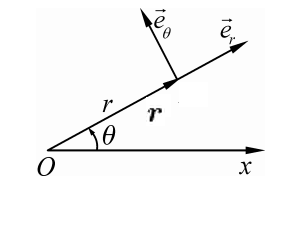
\includegraphics[width=0.9\linewidth]{images/polarbasis.png}
\caption{Basis vectors for polar coordinates}
\label{fig:polarbasis}
\end{wrapfigure}
The basis vectors for polar coordinates are shown in Figure \ref{fig:polarbasis}. To understand why they are defined as such, we should understand the motivation for defining basis vectors and vectors. The motivation is to define velocity. The essence of velocity is to know how an object's coordinates changes after a small amount of time. If a vector is $\vec{v} = 4\hat{e}_x + 3 \hat{e}_y$, it means that after a small amount of time $\Delta t$, the $x$ coordinate changes by $4 \Delta t$, and the $y$ coordinate changes by $3 \Delta t$. This implies that the direction a basis vector (e.g. $\hat{e}_x$) points, is by definition, the direction that the location moves when the coordinate (e.g. $x$) changes.\\[10pt]
For the cartesian coordinate system, the basis vectors are constant: they point in the same direction wherever we are in space. However, the basis vectors for polar coordinates are \textit{not} constant: they point in different directions depending on where we are in space. This is consequential because it implies that the derivative of the basis vectors are not zero, and this mathematical fact gives rise to fictitious/inertial forces such as centrifugal and Coriolis force!\\[10pt]
Enough talking, the expression for basis vectors 
\begin{align}
    \hat{e}_r &=\quad \cos\theta\ \hat{e}_x + \sin\theta\ \hat{e}_y \\
    \hat{e}_\theta &= -\sin\theta\ \hat{e}_x + \cos\theta\ \hat{e}_y
\end{align}

\subsection{Velocity in Polar Coordinates}
The velocity vector can be decomposed into the basis vectors as follows
\begin{align}
    \vec{v} = \dot{r}\ \hat{e}_r + r \dot{\theta}\ \hat{e}_\theta
\end{align}
Proof:
\begin{align}
    \vec{v} &= \frac{d\vec{r}}{dt} \\
    &= \frac{d}{dt} \left(\begin{array}{l}
         x(t) \\
         y(t) 
    \end{array}\right) \\
    &= \frac{d}{dt} \left(\begin{array}{l}
         r(t) \cos \theta(t) \\
         r(t) \sin \theta(t)
    \end{array}\right) \\
    &= \left(\begin{array}{l}
         \dot{r} \cos\theta - r\sin\theta\ \dot\theta \\
         \dot{r} \sin\theta + r\cos\theta\ \dot\theta
    \end{array}\right) \\
    &= \dot{r} \left(\begin{array}{l}
         \cos\theta \\
         \sin\theta
    \end{array}\right) + r \dot{\theta} \left(\begin{array}{l}
         -\sin\theta \\
         \ \cos\theta
    \end{array}\right) \\
    \vec{v} &= \dot{r}\ \hat{e}_r + r \dot{\theta}\ \hat{e}_\theta \label{eq:vpolar}
\end{align}
There are other ways to prove the above, but the above is simplest.
\subsubsection{SJPO 2015 General Round Q4}
Gears A, B, C are aligned side by side in such a way that rotating gear A causes gear $\mathrm{B}$ to rotate which in turn causes gear $\mathrm{C}$ to rotate. Gear A has 40 number of teeth and is rotating at angular speed of $50 \mathrm{rev} / \mathrm{s}$. The radius of gear B is $20 \%$ of gear $\mathrm{C}$ and gear $\mathrm{C}$ is rotating at $40 \%$ angular speed of gear $\mathrm{A}$. All the gears have the same tooth and groove size. How many teeth does gear B have?
\begin{itemize}
\item[] (A) 10
\item[] (B) 20
\item[] (C) 40
\item[] (D) 50
\item[] (E) 80
\end{itemize}
Ans: \ifpaper B \fi
\subsection{Acceleration in Polar Coordinates}
Acceleration is the derivative of velocity (Eq \ref{eq:vpolar}) wrt time, which can be shown to be equal to 
\begin{align}
    \vec{a} = (\ddot{r} - r{\dot\theta}^2)\ \hat{e}_r + (r\ddot\theta + 2\dot r \dot \theta)\ \hat{e}_\theta
\end{align}
When we talk about \textbf{rotating reference frames} in future, the $r{\dot\theta}^2$ term is responsible for \textbf{centrifugal force}, and the $2\dot r \dot \theta$ term is responsible for \textbf{Coriolis force}. \\[10pt]
Proof: First we obtain the derivative of the polar basis vectors.
\begin{align}
    \frac{d\hat{e}_r}{dt} &= \frac{d}{dt}\left(\begin{array}{l}
         \cos\theta \\
         \sin\theta
    \end{array}\right) \\ 
    &= \left(\begin{array}{l}
         -\sin\theta \ \dot\theta  \\
         \ \cos\theta \ \dot\theta 
    \end{array}\right)\\
    &= \dot\theta\ \hat{e}_\theta \\
    \frac{d\hat{e}_\theta}{dt} &= \frac{d}{dt}\left(\begin{array}{l}
         -\sin\theta \\
         \ \cos\theta
    \end{array}\right) \\ 
    &= \left(\begin{array}{l}
         -\cos\theta \ \dot\theta  \\
         - \sin\theta \ \dot\theta 
    \end{array}\right)\\
    &= -\dot\theta\ \hat{e}_r 
    \end{align}
Then we simply apply chain rule
    \begin{align}
    \vec{a} &= \frac{d\vec{v}}{dt} \\
    &= \frac{d}{dt} (\dot{r}\ \hat{e}_r + r \dot{\theta}\ \hat{e}_\theta )\\
    &= \ddot{r}\ \hat{e}_r + \dot{r} \frac{d\hat{e}_r}{dt} + \dot r\dot\theta \ \hat{e}_\theta + r \ddot \theta \ \hat{e}_\theta + r\dot\theta \frac{d\hat{e}_\theta}{dt} \\
    &= (\ddot{r} - r{\dot\theta}^2)\ \hat{e}_r + (r\ddot\theta + 2\dot r \dot \theta)\ \hat{e}_\theta
\end{align}

\section{Physics: Rotational Kinematics in 2D (Polar)}
Newton's 2nd law is just
\begin{align}
    F_r\ \hat{e}_r + F_\theta\ \hat{e}_\theta = \vec{F}_{net} & = m \vec{a} = m \left[(\ddot{r} - r{\dot\theta}^2)\ \hat{e}_r + (r\ddot\theta + 2\dot r \dot \theta)\ \hat{e}_\theta \right]\\
    \Rightarrow F_r &= m(\ddot r - r{\dot\theta}^2) \\ 
    \text{and } F_\theta &= m (r\ddot\theta + 2 \dot r \dot \theta)  
\end{align}
\subsection{Centripetal Acceleration}
Often, the radial coordinate function $r(t)$ is constant. Examples include: pendulum, point mass sliding down hemisphere, planet in orbit, cup on rotating Chinese table. When $\dot r = 0$, Newton's 2nd law simplifies to
\begin{align}
    F_r &= -r {\dot\theta}^2 \\
    F_\theta &= r\ddot\theta
\end{align}
\subsubsection{SJPO 2015 General Round Q1}
Two identical masses, $\mathrm{A}$ and $\mathrm{B}$, are tied to strings and placed on a horizontal frictionless disc as in the figure below. The two masses are then set to move about the centre of the disc with the same angular velocity $\omega$. Given that the tension of the string connecting mass $\mathrm{A}$ to the center of the disc is $T$, determine the tension of the string connecting mass $\mathrm{B}$ to mass $\mathrm{A}$.
\begin{itemize}
\item[] (A) $T / 4$
\item[] (B) $3 T / 4$
\item[] (C) $T$
\item[] (D) $3 T$
\item[] (E) $4 T$
\end{itemize}
Ans: \ifpaper B \fi
\subsubsection{SJPO 2018 General Round Q7}
A bug is just about to slip on a circular turntable of radius $R$ rotating at constant angular velocity. The bug is halfway between the centre and the edge and the coefficient of static friction is $1 / 4$. What is the acceleration of the bug?
\begin{itemize}
\item[] (A) $3 g$
\item[] (B) $2 g$
\item[] (C) $3 g / 2$
\item[] (D) $g / 2$
\item[] (E) $g / 4$
\end{itemize}
Ans: \ifpaper E \fi

\subsubsection{SJPO 2016 General Round Q14}
A ball with mass $m$ is hung from the ceiling with a massless string of length $l$ as shown in the diagram. It moves in uniform circular motion with angular velocity $\omega$. What is the magnitude of tension in the string? \\
{
\begin{wrapfigure}{r}{0.5\textwidth}
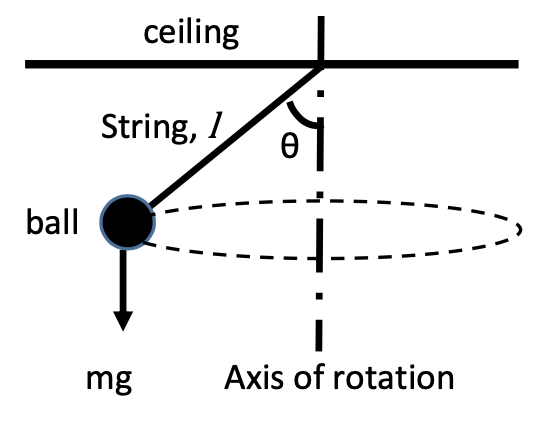
\includegraphics[width=1.0\linewidth]{images/sjpo2016q14.png}
\end{wrapfigure}
\begin{itemize}
\item[] (A) $m \omega^2 l$
\item[] (B) $m \omega^2 l \cos \theta$
\item[] (C) $m \omega^2 l / \cos \theta$
\item[] (D) $m \omega^2 l \sin \theta$
\item[] (E) $m \omega^2 l / \sin \theta$
\end{itemize}
}
Ans: \ifpaper A \fi

\newpage
\subsection{Example: Pendulum}
A mass $m$ is hung by an inextensible string of length $l$ in a gravitational field strength $g$. It is displaced by a small angular displacement $\theta_0$ and released. Find the amplitude and period of oscillation.\\[10pt]
Ans: \\[50pt]
\begin{samepage}
\subsubsection{SJPO 2015 General Round Q16}
As shown in the diagram, a pendulum of length $L$ is hung from the ceiling and at a point $P$, a peg is placed. $L^{\prime}$ denotes the shortened length of the pendulum during part of its oscillation. The period of the pendulums oscillation is now \\
{
\begin{wrapfigure}{r}{0.4\textwidth}
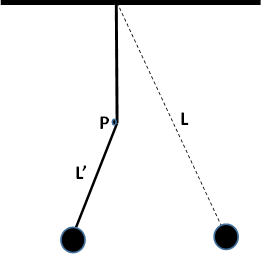
\includegraphics[width=0.9\linewidth]{images/2015q16.png}
\end{wrapfigure}
\begin{itemize}
\item[](A) $2 \pi \sqrt{\frac{L}{g}}$
\item[](B) $2 \pi \sqrt{\frac{L^{\prime}}{g}}$
\item[](C) $2 \pi\left[\sqrt{\frac{L}{g}}+\sqrt{\frac{L^{\prime}}{g}}\right]$
\item[](D) $\pi\left[\sqrt{\frac{L}{g}}+\sqrt{\frac{L^{\prime}}{g}}\right]$
\item[](E) $\pi \sqrt{\frac{L+L^{\prime}}{g}}$
\end{itemize}
Ans: \ifpaper D \fi
}
\end{samepage}

\begin{samepage}
\subsubsection{SJPO 2018 General Round Q21}
The bob of a simple pendulum travels $2 \mathrm{~m}$ in one complete oscillation in a time of $2.000 \mathrm{~s}$. Assuming that damping is negligible, when the same pendulum is made to travel $4 \mathrm{~m}$ in one complete oscillation, the time taken is
\begin{itemize}
\item[](A) $4.000 \mathrm{~s}$
\item[](B) More than $2.000 \mathrm{~s}$
\item[](C) $2.000 \mathrm{~s}$
\item[](D) Less than $2.000 \mathrm{~s}$
\item[](E) $1.000 \mathrm{~s}$
\end{itemize}
Ans: \ifpaper B \fi 
\end{samepage}


\section{Physics: Rotational Dynamics}
So far we have been dealing with point masses. But in reality most objects take up some volume. \\[10pt]
Before we talk about \textit{continuous} mass distributions, let's derive everything using discrete masses first. If there is a mass $m$ distance $r$ away from the origin, rotating about an axis passing through the origin with angular velocity $\omega$.
We usually model these \textbf{rigid body} objects as a uniform mass density over some volume. It is made up of many small masses $dm = \rho dV$, where $dm$ is called an infinitesimal mass element and $dV = dx\ dy\ dz$ is an infinitesimal volume element. If we integral $dm$ over volume $\mathcal{V}$ the object occupies, we get the mass
\begin{align}
    \int_{\mathcal V} dm = m
\end{align}

\subsubsection{SJPO 2018 General Round Q4}
A sphere rolls without slipping down a rough inclined plane. The gain in rotational kinetic energy is due directly to the work done by
\begin{itemize}
\item[](A) Static friction
\item[](B) Kinetic friction
\item[](C) Weight
\item[](D) Normal contact force
\item[](E) Air resistance
\end{itemize}

\section{Physics: Statics}
Need torque
\section{Physics: Springs}
\subsubsection{SJPO 2018 General Round Q19}
Two adventurous Physics students, each weighing $60 \mathrm{~kg}$, jump off a $43 \mathrm{~m}$ high bridge on a Bungee cord. The length of the cord is such that the students together will just touch the water and rebound. While Bungee cords become softer (more elastic) with increasing extension, for our calculations we can approximate the cord as having a constant stiffness of $k=330 \mathrm{~N} / \mathrm{m}$, and we can ignore the height of the students and where the cord is tied on their body. What is the unstretched length of the cord?
\begin{itemize}
\item[] (A) $10.0 \mathrm{~m}$
\item[] (B) $17.5 \mathrm{~m}$
\item[] (C) $25.5 \mathrm{~m}$
\item[] (D) $32.5 \mathrm{~m}$
\item[] (E) $40.0 \mathrm{~m}$
\end{itemize}
\subsubsection{SJPO 2016 General Round Q13}
An ideal uniform spring of mass $m \mathrm{~kg}$, unstretched length $L \mathrm{~m}$ and spring constant $k\  \mathrm{Nm}^{-1}$ stretches by an extension of $x \mathrm{~m}$ when hung vertically. Which statement below is correct? (You may want to know that the sum of $\mathrm{N}$ terms in an arithmetic progression from 1 to $\mathrm{N}$ is $\frac{N(N+1)}{2}$)
\begin{itemize}
\item[] (A) The top half of the spring with mass $\frac{m}{2} \mathrm{~kg}$ has an extension $\frac{x}{2} \mathrm{~m}$.
\item[] (B) The top half of the spring with length $\frac{L+x}{2} \mathrm{~m}$ supports $\frac{m g}{2} \mathrm{~N}$.
\item[] (C) The top half of the spring with mass $\frac{m}{2} \mathrm{~kg}$ has a spring constant of $\frac{k}{2} \mathrm{Nm}^{-1}$.
\item[] (D) The extension of the whole spring is $\frac{m g}{k} \mathrm{~m}$
\item[] (E) The length of the whole spring is $L+\frac{m g}{2 k} \mathrm{~m}$
\end{itemize}
Ans: \ifpaper E \fi

\section{Math: Other Coordinates}
\section{Math: 2D \& 3D Integrals}
\clearpage
\section{Physics: Center of Mass}
\subsubsection{SJPO 2018 General Round Q5}
A thin wire is bent into the form of a three-sided shape as shown below. Each segment has equal length $l$. The height of the centre of mass from the bottom of the shape is \\
{
\begin{wrapfigure}{r}{0.3\textwidth}
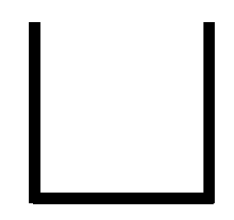
\includegraphics[width=1.0\linewidth]{images/sjpo2018q5.png}
\end{wrapfigure}
\begin{itemize}
\item[] (A) $l / 2$
\item[] (B) $2 l / 3$
\item[] (C) $l / 3$
\item[] (D) $l / 4$
\item[] (E) $2 l / 5$
\end{itemize}
}

\subsubsection{SJPO 2018 General Round Q20}
A dog weighing $10 \mathrm{~kg}$ is standing on a flatboat so that he is $20 \mathrm{~m}$ from the shore. The boat weighs $40 \mathrm{~kg}$ and has uniform mass distribution. The dog walks $8.0 \mathrm{~m}$ on the boat towards the shore and stops. For this calculation, one can assume no friction or drag between the boat and the water. How far is the dog from the shore now? \\
{
\begin{wrapfigure}{r}{0.6\textwidth}
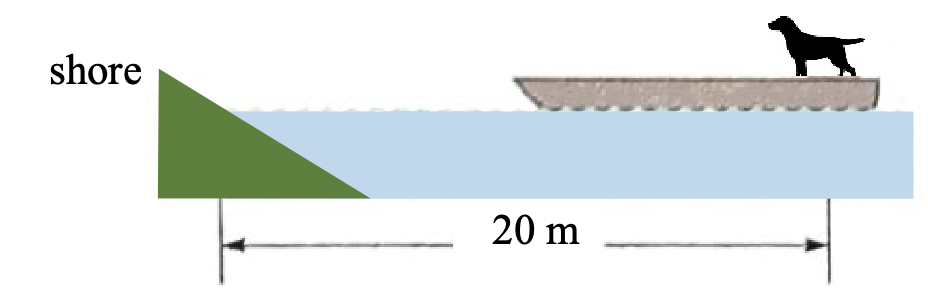
\includegraphics[width=1.0\linewidth]{images/sjpo2018q20.png}
\end{wrapfigure}
\begin{itemize}
\item[] (A) $12.0 \mathrm{~m}$
\item[] (B) $13.6 \mathrm{~m}$
\item[] (C) $14.0 \mathrm{~m}$
\item[] (D) $16.8 \mathrm{~m}$
\item[] (E) $29.8 \mathrm{~m}$
\end{itemize}
}
\clearpage


\section{Physics: Moment of Inertia}
\section{Physics: Electrostatics}

\section{Math: Vector Calculus}
\clearpage
\section{Physics: Potentials \& Potential Energy}
\subsubsection{SJPO 2018 General Round Q1}
The figure shows the potential energy $V(x)$ as a function of molecular separation $x$ for a diatomic molecule of reduced mass $\mu$.
If $V(x)=V_0\left(1-e^{-\left(x-x_0\right)/\delta}\right)^2-V_0$, the vibrational frequency $f$ at the equilibrium position is
(Hint: This series expansion may be useful. $e^x \approx 1+x+\frac{x^2}{2 !}$ ) \\
\begin{wrapfigure}{r}{0.6\textwidth}
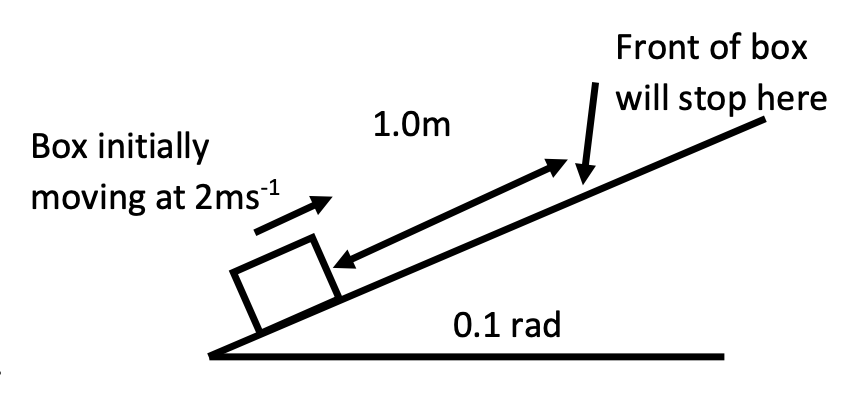
\includegraphics[width=1.0\linewidth]{images/sjpo2016q4.png}
\end{wrapfigure}
\begin{itemize}
\item[] (A) $\frac{2 V_0}{\mu \delta}$
\item[] (B) $\frac{V_0}{2 \pi^2 \mu \delta}$
\item[] (C) $\sqrt{\frac{2 V_0}{\mu \delta^2}}$
\item[] (D) $\frac{1}{2 \pi} \sqrt{\frac{2 V_0}{\mu \delta^2}}$
\item[] (E) $\frac{1}{2 \pi} \sqrt{\frac{V_0}{\mu \delta^2}}$
\end{itemize}
Ans: \ifpaper D \fi
\clearpage
\section{Physics: Electromagnetism}
\section{Physics: AC Circuits}

\section{Math: Differential Equations}
\subsection{SHM: Driven and Damping}
\subsection{Laplace Transform}

\section{Physics: Constraining Forces - Normal, Tension, Friction}
\section{Physics: Pulleys}
\subsection{Friction - Capstan Equation}
\section{Physics: DC Circuits}
\section{Physics: Fluid Mechanics}
\section{Physics: Waves}
\section{Physics: Optics}
\section{Physics: Thermodynamics}
\section{Physics: Non-Inertial Reference Frame}
\subsubsection{SJPO 2018 General Round Q3}
A plumb line is held steady while being carried in a moving train. The mass of the plumb bob is $m$, and the train is accelerating in the forward direction at $0.5 g$. What is the tension in the string?
\begin{itemize}
\item[] (A) $0.5 mg$
\item[] (B) $1.12 mg$
\item[] (C) $1.22 mg$
\item[] (D) $2 mg$
\item[] (E) Cannot be determined from the given information.
\end{itemize}

\end{document}
